% KU defaults
\documentclass[11pt, a4paper]{article}
\usepackage[english, science, titlepage, dropcaps]{ku-frontpage}
\usepackage[utf8]{inputenc}

% Additional packages
\usepackage{lipsum}
\usepackage{cite}
\usepackage[toc,page]{appendix}
\usepackage{listings}
\usepackage{xcolor}
\usepackage{footnote}
\makesavenoteenv{tabular}
\makesavenoteenv{table}

% KU settings
\setlength\arraycolsep{2 pt}
\setcounter{tocdepth}{2}
% \setcounter{secnumdepth}{0}

% User settings
\lstloadlanguages{C,C++,csh,Java}

\usepackage{color}
\definecolor{bluekeywords}{rgb}{0.13,0.13,1}
\definecolor{greencomments}{rgb}{0,0.5,0}
\definecolor{redstrings}{rgb}{0.9,0,0}

\usepackage{listings}
\lstset{language=[Sharp]C,
  showspaces=false,
  showtabs=false,
  breaklines=true,
  showstringspaces=false,
  breakatwhitespace=true,
  escapeinside={(*@}{@*)},
  commentstyle=\color{greencomments},
  keywordstyle=\color{bluekeywords},
  stringstyle=\color{redstrings},
  basicstyle=\ttfamily
}
\usepackage{caption}
\DeclareCaptionFont{white}{\color{white}}
\DeclareCaptionFormat{listing}{\colorbox{blue}{\parbox{\textwidth}{\hspace{15pt}#1#2#3}}}
\captionsetup[lstlisting]{format=listing,labelfont=white,textfont=white, singlelinecheck=false, margin=0pt, font={bf,footnotesize}}

\assignment{Master thesis}
\author{Martin Thiele}

\title{Banking the unbanked}
\subtitle{Future-proofing the least developed countries as they go from cash to online payment}
% \subtitle{Utilizing current technology to bank the unbanked to support the transition from cash to online payment}
\date{Handed in: \today}
\advisor{Advisors: Fritz Henglin, Søren Terp Hørlück Jessen}
\frontpageimage{figs/phonecashheader.jpg}

\begin{document}

\renewcommand{\bibname}{References}


\maketitle

\begin{abstract}
\lipsum[1]
\end{abstract}

\clearpage

\section*{Acknowledgements}
Acknowledge Søren and Fritz, as well as friends and family...

\clearpage

\tableofcontents
\clearpage


\section{Introduction}

% Introduce the problem and why banking is necessary
Financial inclusion is the ability to have access to basic banking which includes efficient and secure transactions, trusted ownership, execution of payments, safe storage of money, and withdrawal of cash. This has been defined by The World Bank to be an important building block for both poverty reduction and opportunities for economic growth\cite{gfindex} and is one of the focal points of many international agencies, such as the International Monetary Fund (IMF)\footnote{\url{https://www.imf.org/en/About/Factsheets/IMF-at-a-Glance}} and The World Bank\footnote{\url{https://www.worldbank.org/en/what-we-do}}, as well as non-profit organizations (NPOs) like the Norwegian Refugee Council (NRC)\footnote{\url{https://www.nrc.no/what-we-do/themes-in-the-field/cash-and-vouchers/}}. By having access to these tools societies will see many benefits. In Niger, a five-month relief program swapped from a monthly payment of cash to instead use mobile money services allowing for mobile commerce (m-commerce). This change saved the recipients 20 hours on average in overall travel and wait time to obtain the payments\cite{gfindex}. A similar study was performed in Kenya where the change to mobile money services allowed 185,000 women-headed households to increase their savings by more than 20\%, reducing extreme poverty among these households by 22\%. Additionally, access to digital payments allows for easier storage and a reduction in corruption in countries where trust in the government is low\cite{gfindex}.

% Statistics
% Statistics - Amount of banked / unbanked
\begin{figure}[ht]
\centering
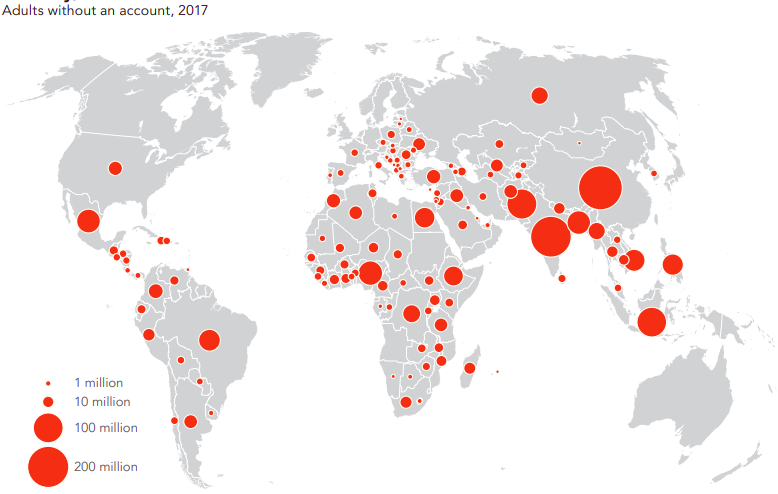
\includegraphics[width=1\linewidth]{figs/unbanked_map}
\caption{\textit{The Global Findex Database}. Map of locations for unbanked adults in 2017.}
\label{fig: unbanked_map}
\end{figure}
\clearpage

The Global Findex Database reports that 69\% of adults in 2017 had a bank account\cite{gfindex}, an increase of 7\% since 2014 and 18\% since 2011\cite{gfindex}. 94\% of adults in developed countries own a bank account, whereas only 63\% of adults own an account in developing countries\cite{gfindex}. Globally, approximately 1.7 billion adults remain unbanked, with half of them living in just seven developing areas: Bangladesh, China, India, Indonesia, Mexico, and Pakistan.

When looking at developing countries and financial technology (fintech) it is important to consider what technologies are available in these areas. 1.1 billion of the financially excluded adults own a mobile phone\cite{gfindex}, however, many developing countries have very little internet access. Our World in Data reports that for the majority of the countries in Sub-Saharan Africa (SSA), one of the least developed regions, the population with access to the internet is only between 5 and 20\%\cite{owidinternet}, however for most of these countries, the mobile phone penetration rate\footnote{The mobile phone penetration rate refers to the amount of SIM cards in a certain country} is greater than 40\%\cite{owidinternet}.

Banking the unbanked is a \$380 billion revenue opportunity\cite{accenture} which has seen an increase in interest throughout the last decade, mainly due to the success M-Pesa has had in Kenya. M-Pesa is a mobile phone-based money transfer service launched in 2007 by the telecommunications company Vodafone Group and the mobile network operator (MNO) Safaricom. M-Pesa utilizes the Unstructured Supplementary Service Data (USSD), also known as "quick codes", a protocol similar to short message service (SMS) with the exception that it creates a connection allowing for a two-way exchange between the parties. Additionally, it doesn't store the messages on the mobile phone. The benefit of using USSD is that it is a feature available in both smartphones and dumbphones\footnote{A mobile device without internet capacity and little computing power}, making it available to every user with a mobile phone. With a mobile phone penetration rate of 103.769\cite{wbinternet} in Kenya, it is safe to assume that most of the citizens are covered.


In this thesis we will take an example-driven approach of defining the needs and requirements of a mobile banking application, as well as determine the best-suited country to onramp such a project, ensuring that the targeted country's needs, likewise, are met. When the requirements are defined we will implement a basic bank meeting these requirements, utilizing the technology that is available to them, with features that allow for any user to see the benefits of entering the mobile bank network. We will then evaluate the use cases of this product, measured up against existing mobile banks, before performing a security analysis looking at the potential attack vectors of the mobile bank. We will then discuss the implementation and reason for our choices before taking a look at the existing work done within this field which we have drawn inspiration from, as well as note what we find, could be a useful next step if this project were to be developed further. Finally, we will conclude with our findings.


\clearpage
\section{Analyzing the needs of a banking service}
\subsection{The regions in need of becoming banked}
\begin{table}[!ht]
\begin{tabular}{|l|l|l|l|}
\hline
\textbf{Region}             & \textbf{Account (\%)} & \textbf{FI\footnote{Financial institution account} account (\%)} & \textbf{M\footnote{Mobile money account} (\%)} \\ \hline
East Asia \& Pacific        & 70.6                  & 70.3                     & 1.3                                \\ \hline
Europe \& Central Asia      & 65.3                  & 65.1                     & 3.2                                \\ \hline
Latin American \& Caribbean & 54.4                  & 53.5                     & 5.3                                \\ \hline
The Middle East \& North Africa & 43.5                  & 43.0                     & 5.8                                \\ \hline
South Asia                  & 69.6                  & 68.4                     & 4.2                                \\ \hline
Sub-Saharan Africa          & 42.6                  & 32.8                     & 20.9                               \\ \hline
\end{tabular}
\caption{Financial inclusion statistics from six regions of the world, aged 15 and up\cite{littledata}}.
\label{tab:financial_statistics}
\end{table}

\noindent We can from \autoref{tab:financial_statistics} and \autoref{fig: unbanked_map} deduce that majority of the financially excluded people are located in the Middle East \& North Africa (MENA) (43.5\%), and Sub-Saharan Africa (SSA) (42.6\%), whereas only 32.8\% of the people in SSA are banked through traditional means. 20.9\% are banked through mobile money accounts, showing a clear need for a fintech (financial technology) solution in these regions. There are many possible approaches to choose from when considering the implementation of a banking system, e.g. Bluetooth-based, blockchain-based, EMV cards (Debit and credit cards). To determine which approach, and which of the two regions has the best infrastructure to support the different approaches we will analyze them based on the following parameters:
\begin{itemize}
     \item \textbf{Mobile penetration rate}

     The amount of active cellular subscriptions in the region
     \item \textbf{Smartphone penetration rate}

     The number of active smartphones in the region
     \item \textbf{Cost of entry-level internet-enabled device}

     The cost of a simple smartphone (in GDP per capita)

     \item \textbf{Data affordability}

     The price for 100 MB of data (in monthly GDP per capita)

     \item \textbf{Mobile infrastructure (Rural)}

     How well the rural parts of the regions are covered by 2G, 3G, and 4G mobile internet.

     \item \textbf{Mobile infrastructure (Urban)}

     How well the urban parts of the regions are covered by 2G, 3G, and 4G mobile internet.

     \item \textbf{Internet download speed}

     \item \textbf{Barriers from being banked}

     \item \textbf{Currently utilized banking services}
 \end{itemize}

\noindent The mobile phone penetration rate was generally between 40-75\% in SSA in 2017, with some countries above 80\% and a few above 120\%\cite{owidinternet}, suggesting that people have more than one cellular subscription. In Africa, this isn't uncommon due to several factors:
\begin{itemize}
    \item Carriers attempt to attract subscribers with special deals, e.g. unlimited SMS, cheaper network calls, bonus monthly data plans\cite{arwhy}.
    \item Costs of services matter a lot, particularly in poor countries, as such swapping between providers can be a lucrative investment\cite{arwhy}.
    \item Network reception might be poor in remote areas of Africa, as such, another network might have better coverage in the given area\cite{arwhy}.
\end{itemize}
In MENA however, the majority of countries have a rate above 100, with only a few countries, such as Iraq, around the 80s.

 The smartphone penetration rate was 45\% in SSA in 2018, with a projected increase to 67\% in 2025. The same rate was 57\% in MENA, with a projected increase to 74\%\cite{gsmame}, suggesting that a smartphone implementation might not meet the requirements that SSA and MENA currently have, since implementing such a system would cut off the majority of its potential users in SSA. An entry-level smartphone in SSA costs 4.6\% GDP per capita and 2.5\% GDP per capita in MENA, making these devices fairly expensive. For comparison, a similar device costs 0.8\% GDP per capita in South America\cite{gsma}.

Internet and the cost of internet data are important factors for any implementation requiring internet, as such data affordability will have to be taken into account. In SSA, 100MB of data costs 4.3\% of the monthly GDP per capita in 2017, a decrease from 2014's 8.6\%. In MENA the same data is 0.7\% of the monthly GDP per capita, which in 2014 was 1.2\%\cite{gsma}. The infrastructure to support the internet in these regions exist, but could be better. In rural Africa, the continent is covered by 22\% 4G internet, 40\% 3G internet, and 18\% 2G internet, making 20\% of rural Africa inaccessible, whereas 77\% of urban Africa is covered by 4G and the last 23\% by 4G. The rural parts of the Arab States, are covered by 44\% 4G internet, 34\% 3G internet and 10\% 2G internet, leaving 12\% of the region inaccessible. Quite similar to Africa, 78\% of the urban Arab States are covered by 4G internet, with the remaining 22\% covered by 3G\cite{ituinternet}. Internet speeds have become better throughout the period of 2014-2017, further closing the gap being the developing countries and the developed ones. In SSA the average download speed was 0.5 Mbps in 2014, which has increased to 2.4 Mbps in 2017. Similarly, MENA has increased from 2.0 Mbps to 7.6 Mbps\cite{gsma}.

To summarize on the infrastructure, both regions have mobile phones available to them and a future of smartphones. SSA and MENA have both progressed well from 2014 to 2017, by providing cheaper data and faster internet. The internet is accessibility is good, with 3G or 4G covered in urban SSA and urban MENA, but with some rural areas not yet covered. With the infrastructure to support at least mobile phones, but not yet ready for smartphones, let's determine why the people aren't banked already.

\begin{table}[!ht]
\centering
\begin{tabular}{|l|l|l|}
\hline
\textbf{Reason} & \textbf{SSA (\%)} & \textbf{MENA (\%)} \\ \hline
Distance to bank & 19 & 5 \\ \hline
Services are too expensive & 19 & 12 \\ \hline
Lack of necessary documentation & 18 & 7 \\ \hline
Lack of trust in financial institutions & 10 & 7 \\ \hline
Religious reasons & 4 & 4 \\ \hline
Insufficient funds & 51 & 44 \\ \hline
A family member has an account & 8 & 7\\ \hline
\end{tabular}
\caption{Reasons for lack of financial accounts in SSA and MENA\cite{gfindex}}
\label{tab:ssa_mena_reasons}
\end{table}

from \autoref{tab:ssa_mena_reasons} we can see that distance is a problem for almost one-fifth of all the unbanked people in SSA, whereas this isn't a major concern for the citizens in MENA.

Service costs are a problem for both regions, but seeing how SSA consists of a lot of developing countries with a poor GDP, it's that SSA leads this statistic.

18\% of SSA lack the identification necessary to become banked, and banks are known to not take such risks. World Bank Group\cite{worldbankid} reasons that people don't have an id due to the fee costs revolving around obtaining one. Often fees can cost upwards of 8-10 US Dollars\cite{worldbankid}, with an additional cost for travel costs and supporting documentation\cite{worldbankid}. Additionally, lack of an id is often not a barrier in the peoples day to day life\cite{worldbankid}.

Both regions lack trust in financial institutions to a lesser degree than the previous reasons, this is understandable for both regions, particularly SSA who have had a history of corrupt governments, to this day, corruption is still at large in some SSA countries. With the COVID-19 pandemic, the trust in governments further increased due to mishandling of funds, overpricing, as well as hoarding of COVID-19 medication\cite{cpi2020}.

4\% in SSA and MENA reason that religious reasons are a cause for them not to be banked. Many countries in SSA and MENA are highly religious but only a few of them list religion as a concern. Niger is a Muslim-dominant country with 98.4\% of the population being Muslim\cite{muslim}. Islamic finance comes with a set of rules which should be in accordance with Islamic law, particularly lending with interest is prohibited since it is deemed exploitative to earn money from interest\cite{islam_invest}.

The majority reason for both regions is the lack of funds to enter a bank, as such, to provide banking services for the poorest people in the world, the service has to be cheap, and there need to be additional reasons for them to become banked.

Lastly, 8\% and 7\% respectively cite that they don't have an account because a family member has one, this can be explained by the service cost of being banked, or because of financial literacy issues. In general, the amount of education in SSA is very low with some countries having less than two years of schooling on average\cite{hdr}. The education level is overall better in MENA\cite{hdr}.

Overall MENA has very few reasons to not be banked other than the lack of funds, what hinders the region from mobile banks however is regulations. Most countries across MENA haven't allowed non-banks to launch mobile money services.\cite{gsmareg}

SSA is already thriving with mobile bank services, particularly M-Pesa in Kenya. Many mobile network operators attempt to replicate the success of M-Pesa, utilizing their already existing mobile network to support USSD, as well as local mom-and-pop shops to act as agents providing the service of depositing and withdrawing. We reason that there are other potential means of providing a banking service with the existing technology available, however, before settling on implementation we will focus our scope on finding a specific country in SSA since the regulations in MENA prohibit non-banks from providing banking services.



\subsection{Determining the best-suited country} % (fold)
\label{sub:determining_the_best_suited_country}
Similar to how we determined the most-suited region, we will take an analytic approach to who has the biggest need, as well as best infrastructure by looking at the following attributes:

\begin{itemize}
  \item Country specifics
  \begin{itemize}
    \item Population size
    \item Surface Area
    \item Population density
  \end{itemize}
  \item Financial specifics
  \begin{itemize}
    \item GDP per capita
    \item Percentage owning a financial institution account
    \item Percentage owning a mobile money account
    \item Percentage financially included
  \end{itemize}
  \item Population specifics
  \begin{itemize}
    \item Average years of schooling
    \item Literacy level
    \item Financial literacy level
    \item Cellular subscriptions
    \item Internet penetration rate
    \item Reasons for being unbanked
  \end{itemize}
\end{itemize}
By comparing the amount of financially included with the average of the region, as well as comparing the number of mobile money accounts with the amount of financially included, we end up with just 11 countries. Notably, we have included Ethiopia due to the low amount of people within the mobile money ecosystem. The financial specifics of these countries can be found in \autoref{tab:financial_statistics_ssa}.

\begin{table}[ht]
\begin{tabular}{|l|l|l|l|}
\hline
\textbf{Country}              & \textbf{M (\%)} & \textbf{FI (\%)} & \textbf{Financial inclusion (\%)} \\ \hline
Burundi                       & 0.7                        & 7.0                                            & 7.0                                  \\ \hline
Central African Republic      & 0.0                        & 13.7                                           & 13.7                                  \\ \hline
Chad                          & 15.2                       & 8.8                                            & 21.8                                 \\ \hline
Congo, Democratic Republic of & 16.1                       & 15.0                                           & 25.8                                  \\ \hline
Ethiopia                      & 0.3                        & 34.8                                           & 34.8                                  \\ \hline
Guinea                        & 13.8                       & 14.6                                           & 23.5                                  \\ \hline
Madagascar                    & 12.1                       & 9.6                                            & 17.9                                  \\ \hline
Mauritania                    & 4.0                        & 19.0                                           & 20.9                                  \\ \hline
Niger                         & 8.7                        & 9.5                                            & 15.5                                  \\ \hline
Sierra Leone                  & 11.0                       & 12.4                                           & 19.8                                  \\ \hline
South Sudan                   & 0.0                        & 8.6                                            & 8.6                                  \\ \hline
\end{tabular}
\caption{Financial inclusion statistics for some of the 11 most financially excluded countries in SSA}
\label{tab:financial_statistics_ssa}
\end{table}

{\color{red} Write about the attributes and how we settled on Guinea, also mention how cash rules here.}


% subsection determining_the_best_suited_country (end)



\section{Design}
\subsection{Determining requirements}
In Guinea, two major mobile money services already exist, namely Orange Money and MTN Mobile Money, they both function similarly to M-Pesa, i.e. a user can use their mobile phone to send money to another user on the network through USSD codes. To exchange cash for e-money and vice versa they visit a local agent, typically a local shop, whereafter the exchange occurs. We identify several concerns with this method:

\begin{enumerate}
  \item To become an agent an upfront capital is required. In the case of M-Pesa, this amounts to \$1600\cite{cgapreq}. 2.04 times the GDP per capita in Kenya\cite{cgapreq}.
  \item An agent has to be a licensed business\cite{cgapreq}.
  \item Agents takes on a large role by having to register users, handle KYC (Know your customer) information and educating users.
  \item Agents face a higher risk of being robbed, particularly in dangerous areas. 25\% of agents in Brazil had been robbed between 2008 and 2011, losing on average \$500 of their own money\cite{cgapreq}.
  \item USSD is encrypted but phone network operators can view all messages, as well as swap phone numbers.\\
\end{enumerate}

Having looked at the concerns of the existing bank services in Guinea, we will now define the requirements which are specific to guinea:

\begin{enumerate}
  \item The product has to be different from existing mobile money services
  \item The product has to be simple to negate the low level of literacy
  \item The product has to be mobile phone-based to utilize the high amount of cellular subscriptions in the country
  \item The product has to be widely available since 30\% of Guineans reasons distance as a problem
  \item The product has to be cheap to account for the 30\% of Guineans reasoning that expense costs are a problem
  \item The product should ideally be able to onboard people without valid identification, since 38\% reason this as a problem
  % \item The product should show elements of trust
  \item The product should either be in french, or support the three languages which more than 15\% of the country speaks: Fula, Malinké, and Susu
\end{enumerate}

Furthermore, we define two additional requirements to support the on-ramping of users and future of banking services:

\begin{enumerate}
  \setcounter{enumi}{7}
  \item The transactions happening in Guinea, and Africa, in general, is currently dominated by cash, whereas in the western world, the majority of them are done through phone applications or the internet, allowing for e-commerce and ease of payment. For this reason, we believe that two products are needed. One to facilitate the current technology of cell phones and one to facilitate the future of payments through internet devices.
  \item A single-player mode has to exist, a reason to be a part of the banking services regardless of how many others use it.
\end{enumerate}

Lastly, we list the important factors for consumer adoption of electronic and mobile payment systems proposed by Mallat\cite{Mallat}, which overlap with some of the already listed requirements.
\begin{enumerate}
  \item The product should show advantages over cash
  \item The product should be convenient
  \item The product should be easy to use
  \item The product should be cheap
  \item The product should be secure
\end{enumerate}

With the problems regarding existing bank services, the requirements specific to Guinea, and the general product requirements in place, we propose a model inspired by the M-Pesa model. As per requirement 8, we facilitate two implementations, one for the currently available technology, and one for the transition from cash to internet-driven payments.

\subsection{Protocol for the current generation of Guineans}
To support current technology we propose a USSD channel with features similar to that of M-Pesa, Orange Money, and MTN Mobile Money with one large distinction - Any user of the service can become an agent, allowing users to exchange cash for e-money, which we will refer to as a \textit{deposit}, similar to how a person would go to a bank and hand over cash in exchange for the amount being added to the users account balance. Conversely, a user can also choose to exchange e-money for cash. We will refer to this as a \textit{withdrawal}. For this, the agent can choose a fee of their choosing which they can modify as they wish. For instance, if they have a monopoly in a given area they can choose whichever fee they like, however for an area with multiple agents, the fee will have to be competitive. When the user and the agent meet to start the exchange, an age-old problem occurs. Namely the problem of synchronism. Who trades first? It's a problem of trust, with no silver bullet. The common solution would be using a neutral third party, an escrow, however, the additional cost of a third person would make the service unattractive, therefore we reason that when a deposit or a withdrawal occurs, the person delivering cash trades first, in the case of a deposit, this would be the user and the agent in the case of a withdrawal. We rationalize this because we only have a history of transactions for one side of the market, namely the e-money transaction.

This modification solves several problems which we find the M-Pesa model has. Particularly, because a user can choose to become an agent at any time, with any amount of cash or e-money, they don't have to meet the capital requirements of M-Pesa. Neither do they have to be a licensed business, instead, this is a risk we, as a banking service, take. The agent's responsibilities are further reduced as they don't have the responsibility of onboarding other users. Lastly, it is up to the agent and the user to settle on a meeting place for the exchange. Ideally, they settle on a public place to reduce the risk of theft, whereas, if they leave an agent-approved store of M-Pesa, they become an easy target.

This modification additionally meets several of the seven requirements we listed above.
1) It's a modification of an existing product.
2) USSD can be difficult at first but given the limited user options and the fact that all options have to be available on a simple cell phone, the actions required by the user are fairly simple. This, however, is one of the reasons why we also facilitate a second implementation, which we will discuss in the next subsection.
3) The USSD technology is available on all devices utilizing the Global System for Mobile Communications (GS
M), which is the most common mobile communications standard.
4) Where the M-Pesa model utilizes brick-and-mortar stores, this model allows for an agent to be an agent anywhere and to meet with users wherever they desire.
5) Two fees play a role in the expenses of this model, one is the agent fee, and the second is the network fee. The agent fee will eventually settle at a low due to market competition, potentially even free if the agent so desire, or if the user can't find a reasonable agent for a deposit, they can take on the agent role of delivering cash for e-money, essentially trading speed for a larger deposit since the user now has to wait for a counterparty willing to exchange with the user. Network fees can be applied, or we as the bank service provider can take the NPO approach of not taking a fee.
6) Lack of identification is one of the biggest deal-breakers and a topic of interest for many researchers worldwide. Luckily there are multiple ways to allow the registration of people without identification. One proven method is to utilize a user's phone data and assess the user based on that, this method is currently utilized by Tala\footnote{\url{https://tala.co}}, a company allowing for the people without a lack of identity to apply for loans. The lack of identification is a problem for traditional banks, it can however be less of a problem for mobile bank services, depending on how risk-averse they are. A study from 2010 showed that the average balance on M-Pesa accounts were \$2.7\cite{mpesastats}, suggesting that the GDP per capita in Kenya was low, but also that most transactions can be considered micropayments (< \$1), allowing the banking service to take a higher risk.
7) Supporting multiple languages is fairly simple, we reason however that at the beginning of its lifespan, a single language is enough to determine whether the product will succeed or not.
8) the USSD protocol can support the current generation, however as the digital divide lessens between SSA and the developed world, internet-enabled devices need to take the charge to allow for a better user experience, better user interface, better access for the illiterate and to allow for e-commerce.
9) Lastly, we argue that single-player features have to exist. The protocol has several in mind but require partnerships with existing companies, stores, or governments to carry out. These include paying bills, buying airtime, which is the credit used for utilizing mobile phones, or paying at local stores.


\subsection{Protocol for the future generation of Guineans}
To support the transition from cash to online payment we propose an android application that acts similarly to that of the USSD protocol explained in the previous subsection. By utilizing an android application we can develop better user interfaces, supporting the needs of the most illiterate people of Guinea. Furthermore, as e-commerce and m-commerce increase as the digital divide is reduced, an internet-enabled application needs to be ready to support these features, allowing any user to see what they purchased, when they purchased it, and for how much.

\subsection{Features}
In total, these protocols will in their basic states allow for 12 features. Here we will list and document how they function through example. Each option starts by either dialing the USSD service code or having logged into the smartphone application.

\begin{enumerate}
  \item \textbf{Transfer money}
  Alice wishes to send 10 Electronic Guinean Franc (E-GNF) to Bob. Alice enters the amount, followed by Bob's phone number. Alice is then prompted to confirm the transfer before finally receiving a receipt for the transfer.
  \item \textbf{Request money}

  Alice wishes to receive 10 E-GNF from Bob. Alice enters the amount, followed by Bob's phone number, and if Alice wishes, she can add a reason for the request. Bob then receives a notification through SMS, the android notification system, or through a network-initiated USSD message. Bob can then choose to accept or decline the request.
  \item \textbf{Deposit money}

  Alice wishes to deposit 10 Guinean Franc (GNF) in exchange for E-GNF, when starting the flow, Alice is presented with a list of agents who is willing to make the exchange. Alice chooses the best-suited agent and accepts their fee charges. Alice receives a confirmation message and a pending transaction has been made. The agent receives a notification notifying them about the pending deposit. We encourage the participant delivering cash to trade first throughout several steps of the flow as the mobile bank service only has an insight on the other half of the transaction. When Alice and the agent have contacted each other and settled on a place to meet, Alice will hand over the cash, where after the agent will confirm the pending transfer.
  \item \textbf{Withdraw money}

  Alice wishes to withdraw 10 GNF in exchange for E-GNF. Alice goes through a list of agents willing to complete this exchange. Alice chooses the best-suited agent and accepts their fee charges. The agent receives a notification about the pending exchange. Both parties can start contact with each other to determine a meeting place to complete the transaction. When the exchange occurs, we encourage the agent to deliver first for the same reasons as mentioned in the deposit money case. When Alice has received the cash, she confirms the pending transfer.
  \item \textbf{View transaction history}

  All users can see their transaction history, which for each transaction, lists the amount, the sender or recipient, the status (pending, completed, or declined), the completion date, and the type (transfer, request, withdrawal, deposit). Due to the character limitations of the USSD protocol, only five transactions can be seen at a time.
  \item \textbf{Confirm pending transactions}

  To confirm a pending transaction, the USSD user will see a list of pending transactions when the option is entered. The user can then enter the id of the transaction before confirming the confirmation by entering their personal PIN code.

  On the android application, the user can instead do this directly from a fold-out option in their transaction history.
  \item \textbf{Decline pending transactions}

  Similarly to confirming a pending transaction, the user will be able to see a list of pending transactions and enter the id to decline the pending transfer. This will not require the entering of a PIN code as the action does not involve the transfer of money.

  The decline option can similarly to the confirm option be found in the transaction history of the android application.

  \item \textbf{View balance}

  \item \textbf{Enable/disable becoming an agent delivering cash}

  If Alice wishes to deliver cash in exchange for e-money, they can sign up as an agent. In this flow, they note how much cash they are willing to exchange in a single transaction, as well as their fee for the service. Now when anyone else wishes to deposit or withdraw, they can request Alice as their agent. To disable this, Alice can use this option again which will immediately disable Alice's agent status.
  \item \textbf{Enable/disable becoming an agent delivering e-money}

  Similar to how a user can sign up as an agent delivering cash, they can do the opposite of delivering e-money.
  \item \textbf{Request help}

  When entering the help menu option, the user is met with an input field and a description, requesting them to ask a question before pressing a button to submit the question. As we don't know which problems will occur, we leave this open-ended, such that we can determine what issues typically arise.
  \item \textbf{Register account}

  Registering an account consists at its core of connecting the phone number to an account. To do this we ask for the user's phone number if they're using the android application, and their PIN code.
\end{enumerate}
with an additional thirteenth and fourteenth for the android application of logging in and out of the service. This is not needed for the USSD protocol as the phone number is sent with the request.

% subsection competition (end)

\section{Implementation}
This implementation is a proof of concept that implements the before-mentioned features, and fulfills the requirements previously discovered. In this section, we will explain the architecture behind the USSD protocol, the android application, and the server that combines them. The complete architecture can be seen in \autoref{fig: sa}

\begin{figure}[ht]
\centering
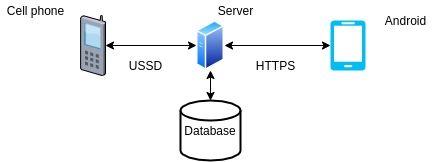
\includegraphics[width=0.7\linewidth]{figs/SA2.png}
\caption{Software Architecture for a proof of concept covering USSD and internet transactions through an android application.}
\label{fig: sa}
\end{figure}
\subsection{Server} % (fold)
We have implemented a fault-tolerant C\# HTTP server which allows for multiple asynchronous connections at a time. This server supports the default operations of GET, PUT, PATCH, POST, DELETE. The server has the features mentioned earlier implemented, with each of the actions involving transaction of money, unit tested to ensure correctness.

\subsubsection{Database}{}
For simplicity, we have created a memory-only database. This database consists of three tables, the user table with the database schematic available in \autoref{tab: user}, the transaction table, with schematics available in \autoref{tab: transaction}, and the question table, with schematics available in \autoref{tab: question}. As this database is stored in memory, it does not uphold the ACID properties.

\begin{table}[ht]
\begin{tabular}{ll}
\hline
\multicolumn{2}{|c|}{\textbf{User}}                                                   \\ \hline
\multicolumn{1}{|l|}{\textbf{Column}}                  & \multicolumn{1}{l|}{\textbf{Data type}} \\ \hline
\multicolumn{1}{|l|}{ID}                & \multicolumn{1}{l|}{Integer} \\ \hline
\multicolumn{1}{|l|}{Phone number}      & \multicolumn{1}{l|}{Integer} \\ \hline
\multicolumn{1}{|l|}{ActiveAgentEMoney} & \multicolumn{1}{l|}{Boolean} \\ \hline
\multicolumn{1}{|l|}{ActiveAgentCash}   & \multicolumn{1}{l|}{Boolean} \\ \hline
\multicolumn{1}{|l|}{EMoneyFee}         & \multicolumn{1}{l|}{Decimal} \\ \hline
\multicolumn{1}{|l|}{CashFee}           & \multicolumn{1}{l|}{Decimal} \\ \hline
\multicolumn{1}{|l|}{MaxAmountEMoney}   & \multicolumn{1}{l|}{Decimal} \\ \hline
\multicolumn{1}{|l|}{MaxAmountCash}     & \multicolumn{1}{l|}{Decimal} \\ \hline
\multicolumn{1}{|l|}{Pin}               & \multicolumn{1}{l|}{Integer} \\ \hline
\end{tabular}
\caption{The database schematic for the user.}
\label{tab: user}
\end{table}

\begin{table}[ht]
\begin{tabular}{ll}
\hline
\multicolumn{2}{|c|}{\textbf{Transaction}}                                                   \\ \hline
\multicolumn{1}{|l|}{\textbf{Column}}& \multicolumn{1}{l|}{\textbf{Data type}} \\ \hline
\multicolumn{1}{|l|}{ID}             & \multicolumn{1}{l|}{Integer} \\ \hline
\multicolumn{1}{|l|}{From (User\_ID)} & \multicolumn{1}{l|}{Integer} \\ \hline
\multicolumn{1}{|l|}{To (User\_ID)}   & \multicolumn{1}{l|}{Integer} \\ \hline
\multicolumn{1}{|l|}{Amount}         & \multicolumn{1}{l|}{Decimal} \\ \hline
\multicolumn{1}{|l|}{Fee}            & \multicolumn{1}{l|}{Decimal} \\ \hline
\multicolumn{1}{|l|}{Type}           & \multicolumn{1}{l|}{String} \\ \hline
\multicolumn{1}{|l|}{Status}         & \multicolumn{1}{l|}{String} \\ \hline
\multicolumn{1}{|l|}{Reason}         & \multicolumn{1}{l|}{String} \\ \hline
\multicolumn{1}{|l|}{Complete\_time}  & \multicolumn{1}{l|}{DateTime} \\ \hline
\end{tabular}
\caption{The database schematic for a transaction.}
\label{tab: transaction}
\end{table}

\begin{table}[ht]
\begin{tabular}{ll}
\hline
\multicolumn{2}{|c|}{\textbf{Question}}                                                   \\ \hline
\multicolumn{1}{|l|}{\textbf{Column}}& \multicolumn{1}{l|}{\textbf{Data type}} \\ \hline
\multicolumn{1}{|l|}{ID}             & \multicolumn{1}{l|}{Integer} \\ \hline
\multicolumn{1}{|l|}{From (User\_ID)} & \multicolumn{1}{l|}{Integer} \\ \hline
\multicolumn{1}{|l|}{Q}   & \multicolumn{1}{l|}{String} \\ \hline
\multicolumn{1}{|l|}{Asked\_time}  & \multicolumn{1}{l|}{DateTime} \\ \hline
\end{tabular}
\caption{The database schematic for a question.}
\label{tab: question}
\end{table}

\subsubsection{USSD API}
A USSD request is sent by the mobile network operator as a POST request with the following parameters:
\begin{itemize}
  \item \textbf{networkCode}

  This won't be relevant as we only operate on a single network.

  \item \textbf{phoneNumber}

  The phone number of the user starting the USSD session

  \item \textbf{serviceCode}

  The code the user has to call to start the USSD session

  \item \textbf{text} or \textbf{input}

  The input the user has entered, each step of the process separated with \textbf{*}. It's a text when it only includes integers, otherwise, it is parsed as an input. A text could look as such: \textit{11*15*5}, and input could look as such: \textit{1*please help me transfer money}.

  \item \textbf{sessionId}

  The unique id of the session created when the user called the USSD service code.
\end{itemize}

When developing to support USSD we will mainly utilize the \textit{phoneNumber} and the \textit{text}. When a user connects to the USSD protocol, they need to be met with a list of possible actions. As such, when the \textit{text} string is empty, we return the following list in string format, such that dumbphones can parse it:
\begin{lstlisting}
"1 - Help \n"+
"2 - Check balance \n"+
"3 - List transactions \n" +
"4 - Transfer money \n"+
"5 - Request money \n"+
"6 - Deposit money \n"+
"7 - Withdraw money \n"+
"8 - Confirm transfer \n"+
"9 - Decline transfer \n"+
"10 - Deliver e-money \n"+
"11 - Deliver cash \n"+
"12 - Sign up";
\end{lstlisting}

By parsing the text input and splitting the inputs we can map the first input to an action on the list. From here we can either continue the process by returning \textit{"CON"} followed by the description of the next page. Otherwise, we use \textit{"END"} followed by the result of their action, e.g. their balance. For each input required by the user, a new description is required. From \autoref{fig: server_transfer} we can see a complete USSD request for a transfer. If the input in the request is valid and parsable, i.e. the amount of a transfer is greater than 0, the recipient exists, etc. The transaction occurs.

\begin{figure}[ht]
\centering
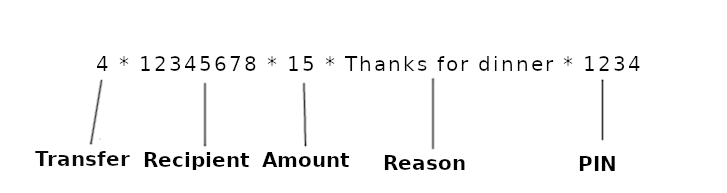
\includegraphics[width=1\linewidth]{figs/transfer_desc.png}
\caption{The input variables and their meaning of a complete USSD request}
\label{fig: server_transfer}
\end{figure}


\subsubsection{Android API}
% subsection server (end)
\subsection{Android}
% subsection android (end)

\section{Evaluation}
\subsection{subsection name} % (fold)
\label{sub:subsection_name}

% subsection subsection_name (end)
\section{Discussion}
\subsection{Related work} % (fold)
\label{sub:related_work}
The concept of mobile banking was first introduced in ... by ... It wasn't until the success of Vodafone Groups M-Pesa in 2007 that the world realized the potential that utilizing existing technology to allow for banking opportunities could lead to a major positive impact on the least developed countries, as well as a major business opportunity. Since 2007...


% subsection related_work (end)
\subsection{Future work} % (fold)
\label{sub:future_work}

% subsection future_work (end)

\subsubsection{Pre-commit} % (fold)
\label{sub:pre_commit}
The implementation for requests, withdrawals, and deposits currently works in 3 stages.
\begin{enumerate}
    \item A request is made for one person to send money to the other.
    \item the requested person and the requesting person meet and trades the cash.
    \item The requested person confirms the request in 1.
\end{enumerate}
This implementation does not take into account whether the requestee has the funds to finish the transfer. A pre-commit would be in order to prove that there is a sufficient amount of funds, thereby reducing theft opportunities.
% subsubsection pre_commit (end)
\subsubsection{Blockchain / Distributed Ledger technology} % (fold)

\label{sub:blockchain_technology}

From {\color{red} section xx} we determined that an E-money license costs {\color{red} xx}, due to the unregulated nature of cryptocurrency it might be easier to work with cryptocurrencies instead. There are additional benefits to this.
\begin{enumerate}
    \item Stablecoins (cryptocurrency typically pegged to the US Dollar) can allow for people in fluctuating economies to enter a stable one.
    \item Cryptocurrency is currently a popular means of investing and is being sought by multiple people.
    \item Cryptocurrencies allow for easy cross-border transfers.
    \item No single point of failure as the data on a distributed ledger is shared between multiple nodes.
\end{enumerate}
The drawbacks however include an increase in fees to countervail the transaction fees of the network, as well as the unknown future and regulations of cryptocurrency

% subsubsection blockchain_technology (end)
\section{Conclusion}

\begingroup
\let\cleardoublepage\clearpage
\addcontentsline{toc}{section}{References}
\bibliographystyle{acm}
\bibliography{thesis}
\endgroup

\begin{appendices}
\section{Source code}
\subsection{Server} % (fold)
% \label{sub:server}
% \begin{lstlisting}
% using System;
% using System.IO;
% using System.Text;
% using System.Net;
% using System.Threading.Tasks;
% using System.Linq;
% using System.Net.Mime;
% using System.Collections.Generic;
% using static System.Net.WebUtility;
% using System.Text.Json;
% using BankTypes;

% namespace HttpListenerBank
% {

%  public static class LingExtension
%  {
%   public static IEnumerable<T> SetValue<T>(this IEnumerable<T> items, Action<T>updateMethod)
%   {
%    foreach (T item in items)
%    {
%     updateMethod(item);
%    }
%    return items;
%   }
%  }


%  class HttpServer
%  {
%   public static HttpListener listener;
%   public static string port = System.Environment.GetEnvironmentVariable("PORT");
%   public static int pageViews = 0;
%   public static bool showRequestInfo = false;
%   public static int requestCount = 0;
%   public static string pageData =
%    "<html>" +
%    "  <head>" +
%    " <style> " +
%    "   table {{border-collapse: collapse}}" +
%    "   table {{min-width: 1000px;}}" +
%    " table tr td {{border: solid 1px #C7C7C7;}}" +
%    " </style>" +
%    "  </head>" +
%    "  <body>" +
%    " {0}" + // account table
%    " <br/><br/>"+
%    " {1}" + // transaction table
%    " <br/><br/>"+
%    " {2}" + // question table
%    " <br/><br/><br/>" +
%    " <form method=\"post\" action=\"reset\">" +
%    "   <input type=\"submit\" value=\"Reset\">" +
%    " </form>" +
%    " <form method=\"post\" action=\"donate\">" +
%    "   <input type=\"submit\" value=\"donate 10 E-GNF to all users\">" +
%    " </form>" +

%    "  </body>" +
%    "</html>";


%   public static List<User> userList = new List<User>() {
%   };

%   public static List<Question> questionList = new List<Question>() {
%   };

%   public static List<Transaction> transactionList = new List<Transaction>() {
%   };

%   // token -> phone number
%   public static Dictionary<string, int> usersLoggedIn = new Dictionary<string, int>(){};


%   private static void reset(){
%    userList = new List<User>(){
% //    new User() { ID = 1, PhoneNumber = 12345678, Balance = 100.0m, ActiveAgentEMoney = true, ActiveAgentCash = true, MaxAmountEMoney = 20, CashFee = 0.05m, EMoneyFee = 0.05m, MaxAmountCash = 25, Pin = 1234} ,
% //    new User() { ID = 2, PhoneNumber = 87654321, Balance = 100.0m, ActiveAgentEMoney = true, ActiveAgentCash = true, MaxAmountEMoney = 200, CashFee = 0.1m, EMoneyFee = 0.1m, MaxAmountCash = 200,  Pin = 1234} ,
%    };
%    transactionList = new List<Transaction>() {
%     // new Transaction() { ID = 1, From = 1, To = 2, Amount = (decimal) 5m, Fee = (decimal) 1.0m, Type = "Deposit", Status = "Complete", Reason = null, Complete_time = DateTime.Now } // User 1 has deposited 5 GNF through User 2. In return user 1 has received 4.95 E-GNF
%      };

%      questionList = new List<Question>(){};

%      usersLoggedIn = new Dictionary<string, int>(){};
%   }



%   private static (int, string) Confirm(int PhoneNumber, int id, int pin){
%    // Find user id
%    User user = userList.SingleOrDefault(u => u.PhoneNumber == PhoneNumber);
%    if(user == null){
%     return (-1, "No user with that phonenumber found");
%    }
%    // Check if correct pin
%    if(user.Pin != pin){
%     return (-1, "Incorrect pin code");
%    }

%    // Fetch transaction
%    try{
%     Transaction transaction = transactionList.SingleOrDefault(t => t.From == user.ID && t.Status == "Pending" && t.ID == id);
%     decimal toTransfer = 0m;
%     if (transaction.Type == "Withdrawal"){
%      toTransfer = transaction.Amount;
%     } else{
%      toTransfer = transaction.Amount - transaction.Amount * transaction.Fee;
%     }
%     if(user.Balance < toTransfer){
%      return (-1, "Invalid funds available to complete transfer");
%     }


%     // Do transfer
%     // Not ACID-proof but for a concept it should be fine
%     if (transaction.Type == "Withdrawal"){
%      // A user would like to withdraw 10 E-GNF worth cash. In order to do so he transfers 10 E-GNF and in return gets 10-10*fee GNF in cash
%      userList.Where(u => u.ID == transaction.From).SetValue(u => u.Balance = u.Balance - transaction.Amount);
%      userList.Where(u => u.ID == transaction.To).SetValue(u => u.Balance = u.Balance + transaction.Amount);
%     } else{
%      userList.Where(u => u.ID == transaction.From).SetValue(u => u.Balance = u.Balance - toTransfer);
%      userList.Where(u => u.ID == transaction.To).SetValue(u => u.Balance = u.Balance + toTransfer);
%     }

%     // Update order to complete
%     transactionList.Where(t => t.ID == transaction.ID).SetValue(t => t.Status = "Complete").SetValue(t => t.Complete_time = DateTime.Now);

%     // Notify sender and recipient that they have confirmed the transaction
%     User from = userList.SingleOrDefault(u => u.PhoneNumber == transaction.From);
%     User to = userList.SingleOrDefault(u => u.PhoneNumber == transaction.To);
%     if(from != null && to != null){
%      var retSender = "";
%      var retRecipient = "";

%      if(transaction.Type == "Transfer"){
%       // Send to sender
%       retSender = $"SMS -> ({from.PhoneNumber}) You have sent {transaction.Amount} E-GNF to {to.PhoneNumber}";
%       if(transaction.Reason != null){
%        retSender+=$". \" {transaction.Reason} \"";
%       }

%       // Send to recipient
%       retRecipient = $"SMS -> ({to.PhoneNumber}) You have received {transaction.Amount} E-GNF from {from.PhoneNumber}";
%       if(transaction.Reason != null){
%        retRecipient+=$". \" {transaction.Reason} \"";
%       }
%      }
%      else if(transaction.Type == "Request"){
%       // Send to sender
%       retSender = $"SMS -> ({from.PhoneNumber}) You have sent the requested {transaction.Amount} E-GNF to {to.PhoneNumber}";
%       if(transaction.Reason != null){
%        retSender+=$". \" {transaction.Reason} \"";
%       }

%       // Send to recipient
%       retRecipient = $"SMS -> ({to.PhoneNumber}) You have received your requested {transaction.Amount} E-GNF from {from.PhoneNumber}";
%       if(transaction.Reason != null){
%        retRecipient+=$". \" {transaction.Reason} \"";
%       }
%      }
%      else if (transaction.Type == "Deposit"){
%       // Send to sender
%       retSender = $"SMS -> ({from.PhoneNumber}) You have delivered {transaction.Amount - (transaction.Amount*transaction.Fee)} E-GNF to {to.PhoneNumber} in exchange for {transaction.Amount} GNF";
%       // Send to recipient
%       retRecipient = $"SMS -> ({to.PhoneNumber}) You have deposited {transaction.Amount} GNF through {from.PhoneNumber}. Your account balance has increased by {transaction.Amount - (transaction.Amount*transaction.Fee)} E-GNF";
%      } else if(transaction.Type == "Withdrawal"){
%       // Send to sender (in this case, the sender is the user, the recipient is the agent)
%       retSender = $"SMS -> ({from.PhoneNumber}) You have withdrawed {transaction.Amount - (transaction.Amount*transaction.Fee)} GNF through {to.PhoneNumber} in exchange for {transaction.Amount} E-GNF";
%       // Send to recipient
%       retRecipient = $"SMS -> ({to.PhoneNumber}) You have delivered {transaction.Amount - (transaction.Amount*transaction.Fee)} GNF to {to.PhoneNumber} in exchange for {transaction.Amount} E-GNF";
%      }
%      Console.WriteLine(retSender);
%      Console.WriteLine(retRecipient);
%     }



%     return (0, "Success");
%    } catch(Exception e){
%     Console.WriteLine(e);
%     return (-1, "Operation failed");
%    }

%   }

%   private static (int, string) Decline(int PhoneNumber, int id){
%    User user = userList.SingleOrDefault(u => u.PhoneNumber == PhoneNumber);
%    if(user == null){
%     return (-1, "No user with that phonenumber found");
%    }
%    // Fetch transaction
%    transactionList.Where(t => t.From == user.ID && t.Status == "Pending" && t.ID == id).SetValue(t => t.Complete_time = DateTime.Now).SetValue(t => t.Status = "Declined");
%    return (0, "");

%   }

%   private static (int, decimal) GetBalance(int PhoneNumber){
%    User user = userList.SingleOrDefault(u => u.PhoneNumber == PhoneNumber);
%    if(user == null){
%     return (-1, 0m);
%    }
%    else {
%     return (0, user.Balance);
%    }
%   }

%   private static (int, List<DTransaction>) ListTransactions(int PhoneNumber, int offset, int amount){
%    try{
%     User user = userList.SingleOrDefault(u => u.PhoneNumber == PhoneNumber);
%     List<Transaction> ts = transactionList.Where(t => t.From == user.ID || t.To == user.ID).OrderByDescending(t => t.Status == "Pending").ThenByDescending(t => t.Complete_time).ToList();
%     ts = ts.Skip(offset).Take(amount).ToList();
%     List<DTransaction> newts = new List<DTransaction>();
%     Dictionary<int, string> dp = new Dictionary<int, string>(); // convert user ids to phone number
%     foreach(Transaction t in ts){
%      DTransaction newT = new DTransaction() {ID = t.ID, From = null, To = null, Amount = t.Amount, Fee = t.Fee, Type = t.Type, Status = t.Status, Reason=t.Reason, Complete_time = t.Complete_time};
%      // convert from ids to phone numbers
%      if (t.From == user.ID){
%       newT.From = "you";
%      } else{
%       if(dp.ContainsKey(t.From)){
%        newT.From = dp[t.From];
%       } else{
%        User u = userList.SingleOrDefault(u => u.ID == t.From);
%        if(u == null){
%         Console.WriteLine($"Tried converting ID to phonenumber for user ID {t.From} but it failed");
%        } else{
%         dp.Add(t.From, u.PhoneNumber.ToString());
%         newT.From = u.PhoneNumber.ToString();
%        }

%       }
%      }


%      // convert to ids to phone numbers
%      if (t.To == user.ID){
%       newT.To = "you";
%      } else{
%       if(dp.ContainsKey(t.To)){
%        newT.To = dp[t.To];
%       } else{
%        User u = userList.SingleOrDefault(u => u.ID == t.To);
%        if(u == null){
%         Console.WriteLine($"Tried converting ID to phonenumber for user ID {t.To} but it failed");
%        } else{
%         dp.Add(t.To, u.PhoneNumber.ToString());
%         newT.To = u.PhoneNumber.ToString();
%        }

%       }
%      }

%      newts.Add(newT);
%     }
%     return (newts.Count, newts);
%    } catch(Exception e){
%     Console.WriteLine(e);
%     return (-1, null);
%    }
%   }

%   private static (int, string) Transfer(int fromphone, int tophone, decimal amount, decimal fee, string type, string reason){
%    User from = userList.SingleOrDefault(u => u.PhoneNumber == fromphone);
%    if(from == null){
%     return (-1, "Sender not found");
%    }
%    User to = userList.SingleOrDefault(u => u.PhoneNumber == tophone);
%    if(to == null){
%     return (-1, "Recipient does not exist");
%    }
%    if(tophone == fromphone){
%     return (-1, "Can't send E-GNF to yourself");
%    }
%    if(amount < 0.0m){
%     return (-1, "Amount can't be negative");
%    }
%    if(amount < 0.1m){
%     return (-1, "Amount can't be less than 0.1 E-GNF");
%    }
%    if(fee < 0.0m){
%     return (-1, "Fee can't be negative");
%    }

%    int TCount = transactionList.Count;
%    Transaction newT = new Transaction() {ID = TCount+1, From = from.ID, To = to.ID, Amount = amount, Fee = fee, Type = type, Status = "Pending", Reason=reason, Complete_time = DateTime.MinValue};
%    try{
%     transactionList.Add(newT);

%     // Notify agent
%     if (type == "Withdrawal"){
%      // Should be an SMS
%      Console.WriteLine($"SMS -> ({to.PhoneNumber}) - User {from.PhoneNumber} has requested {amount-amount*fee} GNF in exchange for {amount} E-GNF");
%     } else if(type == "Deposit"){
%      Console.WriteLine($"SMS -> ({from.PhoneNumber}) - User {to.PhoneNumber} has requested {amount-amount*fee} E-GNF in exchange for {amount} GNF");
%     } else if(type == "Request"){
%      string ret = $"SMS -> ({from.PhoneNumber}) - User {to.PhoneNumber} has requested {amount-amount*fee} E-GNF";
%      if(reason != null && reason != ""){
%       ret+=$". \" {reason} \"";
%      }
%      Console.WriteLine(ret);
%     }
%    } catch(Exception e){
%     Console.WriteLine(e);
%    }
%    return (TCount+1, "");
%   }

%   // The agent marks themselves as available to transfer cash
%   private static (int, string) SetAgentStatusCash(int Phonenumber, decimal MaxAmount, decimal fee){
%    if(MaxAmount < 0.0m){
%     return (-1, "Amount can't be negative");
%    }
%    if(fee < 0.0m){
%     return (-1, "Fee can't be less than 0");
%    }
%    if(fee > 100.0m){
%     return (-1, "Fee can't be greater than 100");
%    }
%    User user = userList.SingleOrDefault(u => u.PhoneNumber == Phonenumber);
%    if(user == null){
%     return (-1, "User not found");
%    }

%    userList.Where(u => u.ID == user.ID)
%     .SetValue(u => u.ActiveAgentCash = !u.ActiveAgentCash)
%     .SetValue(u => u.CashFee = fee/100.0m)
%     .SetValue(u => u.MaxAmountCash = MaxAmount);
%    return (0, "");
%   }

%   private static (int, string) SetAgentStatusEMoney(int Phonenumber, decimal MaxAmount, decimal fee){
%    User user = userList.SingleOrDefault(u => u.PhoneNumber == Phonenumber);
%    if(user == null){
%     return (-1, "User not found");
%    }

%    userList.Where(u => u.ID == user.ID)
%     .SetValue(u => u.ActiveAgentEMoney = !u.ActiveAgentEMoney)
%     .SetValue(u => u.EMoneyFee = fee/100.0m)
%     .SetValue(u => u.MaxAmountEMoney = MaxAmount);
%    return (0, "");
%   }

%   private static int NewUser(int pin, int phone){
%    try{
%     User user = userList.SingleOrDefault(u => u.PhoneNumber == phone);
%     if(user != null){
%      return -1;
%     } else{
%      int UserCount = userList.Count;
%      User newU = new User() {ID = UserCount+1, PhoneNumber = phone, Balance = 0, ActiveAgentEMoney = false, ActiveAgentCash = false, MaxAmountEMoney = 0, MaxAmountCash = 0, Pin = pin};
%      userList.Add(newU);
%      return 0;
%     }
%    } catch(Exception e){
%     Console.WriteLine(e);
%     return -1;
%    }
%   }

%   private static (int, string) newQuestion(int phone, string question){

%    User user = userList.SingleOrDefault(u => u.PhoneNumber == phone);
%    if(user == null){
%     return (-1, "Your phone number could not be found. Are you registered?");
%    }
%    int qCount = questionList.Count;
%    Question newQ = new Question() {ID = qCount+1, From = user.ID, Q = question, Asked_time = DateTime.Now};
%    questionList.Add(newQ);
%    return (0, "Success");
%   }

%   private static void testTransfer(){
%    // Transfer
%    bool testTransfer = true;
%    bool testRequest = true;
%    bool testDeposit = true;
%    bool testWithdraw = true;
%    bool testDecline = true;

%    if(testTransfer){
%     var (id, _) = Transfer(12345678, 87654321, 5m, 0.00m, "Transfer", "For dinner tonight :)");
%     var (_, balgiver) = GetBalance(12345678);
%     var (_, balrecipient) = GetBalance(87654321);
%     Confirm(12345678, id, 1234);
%     decimal expectedGiver = balgiver - 5m;
%     decimal expectedRecipient = balrecipient + 5m;
%     var (_, balgiver2) = GetBalance(12345678);
%     var (_, balrecipient2) = GetBalance(87654321);
%     if (balrecipient2 == expectedRecipient && balgiver2 == expectedGiver){
%      Console.WriteLine("Test (Transfer) - Passed");
%     } else{
%      Console.WriteLine("Test (Transfer) - Failed");
%      Console.WriteLine($"Expected: {expectedRecipient} & {expectedGiver}");
%      Console.WriteLine($"Got {balrecipient2} & {balgiver2}");
%     }
%    }

%    if(testRequest){
%     var (id, _) = Transfer(87654321, 12345678, 5m, 0.00m, "Request", "For dinner tonight :)");
%     var (_, balrecipient) = GetBalance(12345678);
%     var (_, balgiver) = GetBalance(87654321);
%     Confirm(87654321, id, 1234);
%     decimal expectedGiver = balgiver - 5m;
%     decimal expectedRecipient = balrecipient + 5m;
%     var (_, balgiver2) = GetBalance(87654321);
%     var (_, balrecipient2) = GetBalance(12345678);
%     if (balrecipient2 == expectedRecipient && balgiver2 == expectedGiver){
%      Console.WriteLine("Test (Request) - Passed");
%     } else{
%      Console.WriteLine("Test (Request) - Failed");
%      Console.WriteLine($"Expected: {expectedRecipient} & {expectedGiver}");
%      Console.WriteLine($"Got {balrecipient2} & {balgiver2}");
%     }
%    }

%    // Deposit
%    if(testDeposit){
%     decimal amount = 10m;
%     decimal fee = 0.05m;
%     var (b1, baluser) = GetBalance(12345678);
%     var (b2, balagent) = GetBalance(87654321);
%     var (id, _) = Transfer(87654321, 12345678, amount, fee, "Deposit", null);
%     Confirm(87654321, id, 1234);
%     var (b5, baldepositUser) = GetBalance(12345678);
%     var (b6, baldepositAgent) = GetBalance(87654321);
%     decimal expectedUser = baluser + (amount-(amount*fee));
%     decimal expectedAgent = balagent - (amount-(amount*fee));
%     if (baldepositAgent == expectedAgent && baldepositUser == expectedUser){
%      Console.WriteLine("Test (Deposit) - Passed");
%     } else{
%      Console.WriteLine("Test (Deposit) - Failed");
%      Console.WriteLine($"Expected: {expectedAgent} & {expectedUser}");
%      Console.WriteLine($"Got {baldepositAgent} & {baldepositUser}");
%     }
%    }

%    // Withdrawal
%    if(testWithdraw){
%     decimal amount = 10m;
%     decimal fee = 0.05m;
%     var (_, baluser) = GetBalance(12345678);
%     var (_, balagent) = GetBalance(87654321);
%     var (id, _) = Transfer(12345678, 87654321, amount, fee, "Withdrawal", null);
%     Confirm(12345678, id, 1234);
%     var (_, baldepositUser) = GetBalance(12345678);
%     var (_, baldepositAgent) = GetBalance(87654321);
%     decimal expectedUser = baluser - amount;
%     decimal expectedAgent = balagent + amount;
%     if (baldepositAgent == expectedAgent && baldepositUser == expectedUser){
%      Console.WriteLine("Test (Withdrawal) - Passed");
%     } else{
%      Console.WriteLine("Test (Withdrawal) - Failed");
%      Console.WriteLine($"Expected: {expectedAgent} & {expectedUser}");
%      Console.WriteLine($"Got {baldepositAgent} & {baldepositUser}");
%     }
%    }

%    if(testDecline){
%     decimal amount = 10m;
%     decimal fee = 0m;
%     var (_, baluser) = GetBalance(12345678);
%     var (_, balagent) = GetBalance(87654321);
%     var (id, _) = Transfer(12345678, 87654321, amount, fee, "Transfer", "yay");
%     Decline(12345678, id);
%     var (_, baldepositUser) = GetBalance(12345678);
%     var (_, baldepositAgent) = GetBalance(87654321);
%     decimal expectedUser = baluser;
%     decimal expectedAgent = balagent;
%     if (baldepositAgent == expectedAgent && baldepositUser == expectedUser){
%      Console.WriteLine("Test (Decline) - Passed");
%     } else{
%      Console.WriteLine("Test (Decline) - Failed");
%      Console.WriteLine($"Expected: {expectedAgent} & {expectedUser}");
%      Console.WriteLine($"Got {baldepositAgent} & {baldepositUser}");
%     }
%    }
%   }

%   private static string formatUserHtml(){
%    string ret = "<h1>Users</h1>"+
%    "<table id='uTable'>"+
%    " <thead>"+
%    "  <tr>"+
%    "   <td><b>ID</b></td>"+
%    "   <td><b>Phone number</b></td>"+
%    "   <td><b>Balance</b></td>"+
%    "   <td><b>Agent (cash)</b></td>"+
%    "   <td><b>Agent fee (cash)</b></td>"+
%    "   <td><b>Max amount (cash)</b></td>"+
%    "   <td><b>Agent (E-money)</b></td>"+
%    "   <td><b>Agent fee (E-money)</b></td>"+
%    "   <td><b>Max amount (E-money)</b></td>"+
%    "  </tr>"+
%    "  </thead>"+
%    "<tbody>";
%    foreach (User user in userList){
%     ret+=$"<tr>"+
%      $"<td>{user.ID}</td>"+
%      $"<td>{user.PhoneNumber}</td>"+
%      $"<td>{user.Balance}</td>"+
%      $"<td>{user.ActiveAgentCash}</td>"+
%      $"<td>{user.CashFee}</td>"+
%      $"<td>{user.MaxAmountCash}</td>"+
%      $"<td>{user.ActiveAgentEMoney}</td>"+
%      $"<td>{user.EMoneyFee}</td>"+
%      $"<td>{user.MaxAmountEMoney}</td>"+
%      "</tr>";
%    }
%    ret+="</tbody></table>";
%    return ret;
%   }
%   private static string formatTransactionHtml(){
%    string ret = "<h1>Transactions</h1><table id='tTable'><thead><tr>" +

%    "<td><b>ID</b></td>" +
%    "<td><b>From</b></td>" +
%    "<td><b>To</b></td>"+
%    "<td><b>Amount</b></td>"+
%    "<td><b>Fee</b></td>"+
%    "<td><b>Sent</b></td>"+
%    "<td><b>Received</b></td>"+
%    "<td><b>Reason</b></td>"+
%    "<td><b>Type</b></td>"+
%    "<td><b>Status</b></td>"+
%    "<td><b>Complete time</b></td>"+

%    "</tr></thead><tbody>";
%    foreach (Transaction t in transactionList){
%     decimal sent = t.Amount - t.Amount*t.Fee;
%     decimal received = 0.00m;
%     string sentstr = "";
%     string recstr = "";
%     if(t.Type == "Deposit"){
%      sentstr = $"{(t.Amount - (t.Amount*t.Fee))} E-GNF";
%      recstr = $"{t.Amount} GNF";
%     } else if(t.Type == "Withdrawal"){
%      sentstr = $"{t.Amount} E-GNF";
%      recstr = $"{(t.Amount - (t.Amount*t.Fee))} GNF";
%     } else{
%      sentstr = $"{sent} E-GNF";
%      recstr = $"{received} GNF";
%     }

%     ret+=$"<tr>"+

%     $"<td>{t.ID}</td>"+
%     $"<td>{t.From}</td>" +
%     $"<td>{t.To}</td>" +
%     $"<td>{t.Amount}</td>" +
%     $"<td>{t.Fee}</td>" +
%     $"<td>{sentstr}</td>" +
%     $"<td>{recstr}</td>" +
%     $"<td>{t.Reason}</td>" +
%     $"<td>{t.Type}</td>" +
%     $"<td>{t.Status}</td>" +
%     $"<td>{t.Complete_time}</td>" +

%     "</tr>";
%    }
%    ret+="</tbody></table>";
%    return ret;
%   }

%   private static string formatQuestionHtml(){
%    string ret = "<h1>Questions</h1><table id='tTable'><thead><tr>" +

%    "<td><b>ID</b></td>" +
%    "<td><b>From</b></td>" +
%    "<td><b>Question</b></td>"+
%    "<td><b>When asked</b></td>"+

%    "</tr></thead><tbody>";
%    foreach (Question q in questionList){
%     ret+=$"<tr>"+

%     $"<td>{q.ID}</td>"+
%     $"<td>{q.From}</td>" +
%     $"<td>{q.Q}</td>" +
%     $"<td>{q.Asked_time}</td>" +

%     "</tr>";
%    }
%    ret+="</tbody></table>";
%    return ret;
%   }
















%   // USD
%   public static string handleUSSD(Dictionary<String, String> data){

%    string reqText = "";
%    if(data.ContainsKey("text")){
%     reqText = data["text"];
%    } else if(data.ContainsKey("input")){
%     reqText = data["input"];
%    } else{
%     return "END No form data could be found";
%    }
%    int reqPhone = int.Parse(data["phoneNumber"].Remove(0,3)); // remove +45 for danish numbers. Good enough for proof of concept
%    string[] sections = reqText.Split('*');
%    string section = sections[0];
%    int reqlen = sections.Length;
%    switch(section){
%     case "":
%      string response = "CON "+
%        "1 - Help \n"+
%        "2 - Check balance \n"+
%        "3 - List transactions \n" +
%        "4 - Transfer money \n"+
%        "5 - Request money \n"+
%        "6 - Deposit money \n"+
%        "7 - Withdraw money \n"+
%        "8 - Confirm transfer \n"+
%        "9 - Decline transfer \n"+
%        "10 - Deliver e-money \n"+
%        "11 - Deliver cash \n"+
%        "12 - Sign up";
%      return response;
%     case "1": // help
%      if(reqlen == 1){
%       return "CON enter a question and we'll get back to you. If you'd like for us to call you, leave this space empty";
%      } else{
%       var (err, msg) = newQuestion(reqPhone, sections[1]);
%       if(err == -1) {
%        return $"END {msg}";
%       } else{
%        return $"END Your question has been sent. You'll get a response shortly";
%       }
%      }
%     case "2": // balance
%     {
%      var (err, bal) = GetBalance(reqPhone);
%      if(err == 0){
%       return $"END Your balance is: {bal.ToString()} E-GNF";
%      } else{
%       return $"END Something went wrong. Have you signed up?";
%      }
%     }
%     case "3": // list transactions
%      if(reqlen == 1){
%       User user = userList.SingleOrDefault(u => u.PhoneNumber == reqPhone);
%       if(user == null){
%        return "END Your phone number could not be found. Are you registered?";
%       }
%       return "CON Please enter the order offset. 0 if you would like to see the 5 latest transactions. 5 if you'd like to see the 5 afterwards, 10 for the following 5 and so on.";
%      } else{
%       var (amount, ts) = ListTransactions(reqPhone, int.Parse(sections[1]), 5);
%       if(amount == -1){
%        return $"END Something went wrong. Have you signed up?";
%       } else{
%        if(amount == 0){
%         return "END No transactions found";
%        } else{
%         string ret = "END "; //$"END {"From - To - Amount - Fee - Type"} \n";
%         foreach(DTransaction t in ts){
%          if(t.Complete_time != DateTime.MinValue){
%           ret+=$"{t.Complete_time.ToString("dd-MM")} : ";
%          }
%          if(t.Type == "deposit"){
%           ret+=$"{t.From} -> {t.To}. {t.Amount - t.Amount*t.Fee} E-GNF ({t.Type}) [{t.Status}]"; // 02-05 : you -> 12345678. 1.23 GNF (Transfer) [Completed] "Cinema"
%          } else{
%           ret+=$"{t.From} -> {t.To}. {t.Amount} E-GNF ({t.Type}) [{t.Status}]"; // 02-05 : you -> 12345678. 1.23 GNF (Transfer) [Completed] "Cinema"
%          }
%          if(t.Reason != null && t.Reason != ""){
%           ret+=$" \"{t.Reason}\"";
%          }
%          ret+="\n";
%         }
%         return ret;
%        }
%       }
%      }
%     case "4": // transfer
%      switch(reqlen){
%       case 1:
%        User user = userList.SingleOrDefault(u => u.PhoneNumber == reqPhone);
%        if(user == null){
%         return "END Your phone number could not be found. Are you registered?";
%        }
%        return "CON Please enter the phone number of the recipient";
%       case 2:
%        return $"CON Please enter the amount of E-GNF you'd like to send to {sections[1]}";
%       case 3:
%        return $"CON Please enter the reason for the transfer. e.g. dinner or bill. Enter 0 if you'd like to not provide a reason";
%       case 4:
%        return $"CON Please complete your transfer of {sections[2]} E-GNF to {sections[1]} by entering your PIN. Enter 0 to cancel";
%       case 5:
%        if(sections[4] == "0"){
%         return $"END You've declined the transfer of {sections[2]} E-GNF to {sections[1]}";
%        } else{
%         int phone;
%         decimal amount;
%         int pin;
%         string reason = sections[3];
%         bool successPh = int.TryParse(sections[1], out phone);
%         bool successAm = decimal.TryParse(sections[2], out amount);
%         bool successPin = int.TryParse(sections[4], out pin);
%         if(!successPh){
%          return $"END {sections[1]} is not a valid phone number";
%         }
%         if(!successAm){
%          return $"END {sections[2]} is not a valid amount";
%         }
%         if(!successPin){
%          return $"END {sections[4]} is not a valid PIN";
%         }
%         var (id, msg) = Transfer(reqPhone, phone, amount, 0m, "Transfer", reason != "0" ? reason : null);
%         if(id == -1){
%          return $"END {msg}";
%         } else{
%          var (err, msg2) = Confirm(reqPhone, id, pin);
%          if(err == -1){
%           return $"END {msg2}";
%          }
%         }
%         return $"END You've completed the transfer of {sections[2]} E-GNF to {sections[1]}";
%        }
%       default:
%        break;
%      }
%      break;
%     case "5": // request
%      switch(reqlen){
%       case 1:
%        User user = userList.SingleOrDefault(u => u.PhoneNumber == reqPhone);
%        if(user == null){
%         return "END Your phone number could not be found. Are you registered?";
%        }
%        return "CON Please enter the phone number of the person you'd like to request money from";
%       case 2:
%        return $"CON Please enter the amount of E-GNF you'd like to request from {sections[1]}";
%       case 3:
%        return $"CON Please enter the reason for the transfer. e.g. dinner or bill. Enter 0 if you'd like to not provide a reason";
%       case 4:
%        int phone;
%        decimal amount;
%        bool successPh = int.TryParse(sections[1], out phone);
%        bool successAm = decimal.TryParse(sections[2], out amount);
%        string reason = sections[3];
%        if(!successPh){
%         return $"END {sections[1]} is not a valid phone number";
%        }
%        if(!successAm){
%         return $"END {sections[2]} is not a valid amount";
%        }
%        var (id, msg) = Transfer(phone, reqPhone, amount, 0m, "Request", (reason != "0" && reason != "") ? reason : null);
%        if(id == -1){
%          return $"END {msg}";
%        } else{
%         return $"END You've requested {sections[2]} E-GNF from {sections[1]}";
%        }
%      }
%      break;
%     case "6": // Deposit
%      switch(reqlen){
%       case 1:
%       {
%        User user = userList.SingleOrDefault(u => u.PhoneNumber == reqPhone);
%        if(user == null){
%         return "END Your phone number could not be found. Are you registered?";
%        }
%        return "CON Please enter the amount of GNF you'd like to deposit";
%       }
%       case 2:
%       {
%        decimal amount;
%        bool success = decimal.TryParse(sections[1], out amount);
%        if(!success){
%         return "END The amount you entered was invalid. Please start over";
%        }
%        var agents = userList.Where(u => u.ActiveAgentEMoney && amount <= u.MaxAmountEMoney && u.PhoneNumber != reqPhone).Select(u => new {u.ID, u.PhoneNumber, u.EMoneyFee, u.MaxAmountEMoney}).OrderBy(u => u.EMoneyFee).ToList();
%        if(agents.Count > 0){
%         string ret = "CON Please choose an agent by their phone number\nFee - Phone - You will receive\n";
%         foreach(var a in agents){
%          ret+=$"{a.EMoneyFee*100m}% - {a.PhoneNumber} - {amount - (amount*a.EMoneyFee)} E-GNF\n";
%         }
%         return ret;
%        } else{
%         return $"END No agents delivering E-GNF could be found within the amount of {amount}";
%        }
%       }
%       case 3:
%       {
%        decimal amount = decimal.Parse(sections[1]);
%        int agentPhone = int.Parse(sections[2]);
%        User agent = userList.SingleOrDefault(u => u.PhoneNumber == agentPhone && u.ActiveAgentEMoney && amount <= u.MaxAmountEMoney && u.PhoneNumber != reqPhone);
%        if(agent == null){
%         return $"END The requested agent ({agentPhone}) could not be found or is not registered as an agent accepting {amount} GNF";
%        }
%        var (err, msg) = Transfer(agent.PhoneNumber, reqPhone, amount, agent.EMoneyFee, "Deposit", null);
%        if(err == -1){
%         return $"END {msg}";
%        }
%        return $"END You've requested {amount-amount*agent.EMoneyFee} E-GNF from {agent.PhoneNumber} in exchange for your {amount} GNF. Please meet and deliver the agent your GNF";
%       }
%      }
%      break;
%     case "7": // withdraw
%      switch(reqlen){
%       case 1:
%       {
%        User user = userList.SingleOrDefault(u => u.PhoneNumber == reqPhone);
%        if(user == null){
%         return "END Your phone number could not be found. Are you registered?";
%        }
%        return "CON Please enter the amount of GNF you'd like to withdraw";
%       }
%       case 2:
%       {
%        decimal amount;
%        bool success = decimal.TryParse(sections[1], out amount);
%        if(!success){
%         return "END The amount you entered was invalid. Please start over";
%        }
%        var agents = userList.Where(u => u.ActiveAgentCash && amount <= u.MaxAmountCash && u.PhoneNumber != reqPhone).Select(u => new {u.ID, u.PhoneNumber, u.CashFee, u.MaxAmountCash}).OrderBy(u => u.CashFee).ToList();
%        if(agents.Count > 0){
%         string ret = "CON Please choose an agent by their phone number\nFee - Phone - You will receive\n";
%         foreach(var a in agents){
%          ret+=$"{a.CashFee*100m}% - {a.PhoneNumber} - {amount-(amount*a.CashFee)} GNF\n";
%         }
%         return ret;
%        } else{
%         return $"END No agents delivering E-GNF could be found within the amount of {amount}";
%        }
%       }
%       case 3:
%       {
%        decimal amount = decimal.Parse(sections[1]);
%        int agentPhone = int.Parse(sections[2]);
%        User agent = userList.SingleOrDefault(u => u.PhoneNumber == agentPhone && u.ActiveAgentCash && amount <= u.MaxAmountCash && u.PhoneNumber != reqPhone);
%        if(agent == null){
%         return $"END The requested agent ({agentPhone}) could not be found or is not registered as an agent accepting {amount} GNF";
%        }
%        var (err, msg) = Transfer(reqPhone, agent.PhoneNumber, amount, agent.CashFee, "Withdrawal", null);
%        if(err == -1){
%         return $"END {msg}";
%        }
%        return $"END You've requested {amount-amount*agent.CashFee} GNF from {agent.PhoneNumber} in exchange for your {amount} E-GNF. Please meet and receive your GNF from the agent before confirming the transaction";
%       }
%      }
%      break;
%     case "8": // confirm
%      switch(reqlen){
%       case 1: // List transactions pending confirmation
%       {
%        User u = userList.SingleOrDefault(u => u.PhoneNumber == reqPhone);
%        if(u == null){
%         return "END Your phone number could not be found. Are you registered?";
%        }
%        List<Transaction> ts = transactionList.Where(t => t.Status == "Pending" && t.From == u.ID).ToList();
%        if(ts.Count == 0){
%         return "END No transactions are awaiting your confirmation";
%        } else{
%         ts = ts.Take(5).ToList();
%         Dictionary<int, string> dp = new Dictionary<int, string>(); // convert user ids to phone number
%         string ret = "CON please enter the [ID] of the order you'd like to confirm\n";
%         foreach(Transaction t in ts){
%          if(dp.ContainsKey(t.To)){
%           if(t.Type == "Deposit"){
%            ret+=$"[{t.ID}] you -> {dp[t.To]}. {t.Amount-(t.Amount*t.Fee)} E-GNF ({t.Type})";
%           } else{
%            ret+=$"[{t.ID}] you -> {dp[t.To]}. {t.Amount} E-GNF ({t.Type})";
%           }
%          } else{
%           User rec = userList.SingleOrDefault(u => u.ID == t.To);
%           if(rec == null){
%            Console.WriteLine($"Recipient could not be found. ID: {t.ID}. Recipient ID: {t.To}");
%            continue;
%           }
%           dp.Add(t.To, rec.PhoneNumber.ToString());
%           if(t.Type == "Deposit"){
%            ret+=$"[{t.ID}] you -> {rec.PhoneNumber}. {t.Amount-(t.Amount*t.Fee)} E-GNF ({t.Type})";
%           } else{
%            ret+=$"[{t.ID}] you -> {rec.PhoneNumber}. {t.Amount} E-GNF ({t.Type})";

%           }
%          }
%          if(t.Reason != null && t.Reason != ""){
%           ret+=$". \" {t.Reason} \"";
%          }
%          ret+="\n";
%         }
%         return ret;
%        }
%       }
%       case 2: // Enter ID
%       {
%        int id;
%        bool success = int.TryParse(sections[1], out id);
%        if(!success){
%         return $"END {sections[1]} is not a valid ID.";
%        }
%        User u = userList.SingleOrDefault(u => u.PhoneNumber == reqPhone);
%        if(u == null){
%         return "END Your phone number could not be found. Are you registered?";
%        }
%        Transaction t = transactionList.SingleOrDefault(t => t.ID == id && t.From == u.ID && t.Status == "Pending");
%        if(t == null){
%         return $"END no transaction with ID {id} could be found";
%        }
%        User rec = userList.SingleOrDefault(u => u.ID == t.To);
%        if(rec == null){
%         return $"END The recipient of the E-GNF could not be found";
%        }
%        if(t.Type == "Withdrawal"){ // user confirms a withdrawal
%         return $"CON please enter your PIN to verify the transfer of {t.Amount} E-GNF to {rec.PhoneNumber} in exchange for {t.Amount-(t.Amount*t.Fee)} GNF";
%        } else if(t.Type == "Deposit"){ // agent confirms a deposit
%         return $"CON please enter your PIN to verify the transfer of {t.Amount-(t.Amount*t.Fee)} E-GNF to {rec.PhoneNumber} in exchange for {t.Amount} GNF";
%        } else if(t.Type == "Request"){
%         return $"CON please enter your PIN to verify the transfer of {t.Amount} E-GNF to {rec.PhoneNumber}";
%        } else{
%         return $"END Unable to confirm a transaction of type {t.Type}";
%        }
%       }
%       case 3: // Enter PIN
%       {
%        int id;
%        int pin;
%        bool success = int.TryParse(sections[1], out id);
%        bool successPin = int.TryParse(sections[2], out pin);
%        if(!success){
%         return $"END {sections[1]} is not a valid ID.";
%        }
%        if(!successPin){
%         return $"END {sections[2]} is not a valid PIN.";
%        }
%        User u = userList.SingleOrDefault(u => u.PhoneNumber == reqPhone);
%        if(u == null){
%         return "END Your phone number could not be found. Are you registered?";
%        }
%        Transaction t = transactionList.SingleOrDefault(t => t.ID == id && t.From == u.ID && t.Status == "Pending");
%        if(t == null){
%         return $"END no transaction with ID {id} could be found";
%        }
%        User rec = userList.SingleOrDefault(u => u.ID == t.To);
%        if(rec == null){
%         return $"END The recipient of the E-GNF could not be found";
%        }
%        var (err, msg) = Confirm(reqPhone, id, pin);
%        if(err == -1){
%         return $"END {msg}";
%        } else{
%         if(t.Type == "Withdrawal"){ // user confirms a withdrawal
%          return $"END You have completed the transfer of {t.Amount} E-GNF to {rec.PhoneNumber} in exchange for {t.Amount-(t.Amount*t.Fee)} GNF";
%         } else if(t.Type == "Deposit"){ // agent confirms a deposit
%          return $"END You have completed the transfer of {t.Amount-(t.Amount*t.Fee)} E-GNF to {rec.PhoneNumber} in exchange for {t.Amount} GNF";
%         } else if(t.Type == "Request"){
%          return $"END You have completed the transfer of {t.Amount} E-GNF to {rec.PhoneNumber}";
%         }
%         else{
%          return $"END Unable to confirm a transaction of type {t.Type}";
%         }
%        }
%       }
%      }
%      break;
%     case "9":
%      switch(reqlen){ // decline
%       case 1: // List transactions pending declining
%       {
%        User u = userList.SingleOrDefault(u => u.PhoneNumber == reqPhone);
%        if(u == null){
%         return "END Your phone number could not be found. Are you registered?";
%        }
%        List<Transaction> ts = transactionList.Where(t => t.Status == "Pending" && t.From == u.ID).ToList();
%        if(ts.Count == 0){
%         return "END No transactions are awaiting your declining";
%        } else{
%         ts = ts.Take(5).ToList();
%         Dictionary<int, string> dp = new Dictionary<int, string>(); // convert user ids to phone number
%         string ret = "CON please enter the [ID] of the order you'd like to decline\n";
%         foreach(Transaction t in ts){
%          if(dp.ContainsKey(t.To)){
%           ret+=$"[{t.ID}] you -> {dp[t.To]}. {t.Amount} E-GNF ({t.Type})";
%          } else{
%           User rec = userList.SingleOrDefault(u => u.ID == t.To);
%           if(rec == null){
%            Console.WriteLine($"Recipient could not be found. ID: {t.ID}. Recipient ID: {t.To}");
%            continue;
%           }
%           dp.Add(t.To, rec.PhoneNumber.ToString());
%           ret+=$"[{t.ID}] you -> {rec.PhoneNumber}. {t.Amount} E-GNF ({t.Type})";
%          }
%          if(t.Reason != null && t.Reason != ""){
%           ret+=$". \" {t.Reason} \"";
%          }
%          ret+="\n";
%         }
%         return ret;
%        }
%       }
%       case 2: // Enter ID
%       {
%        int id;
%        bool success = int.TryParse(sections[1], out id);
%        if(!success){
%         return $"END {sections[1]} is not a valid ID.";
%        }
%        User u = userList.SingleOrDefault(u => u.PhoneNumber == reqPhone);
%        if(u == null){
%         return "END Your phone number could not be found. Are you registered?";
%        }
%        Transaction t = transactionList.SingleOrDefault(t => t.ID == id && t.From == u.ID && t.Status == "Pending");
%        if(t == null){
%         return $"END no transaction with ID {id} could be found";
%        }
%        User rec = userList.SingleOrDefault(u => u.ID == t.To);
%        if(rec == null){
%         return $"END The recipient of the E-GNF could not be found";
%        }
%        var (err, msg) = Decline(reqPhone, id);
%        if(err == -1){
%         return $"END {msg}";
%        } else{
%         if(t.Type == "Withdrawal"){ // user declines a withdrawal
%          return $"END You have declined the transfer of {t.Amount} E-GNF to {rec.PhoneNumber} in exchange for {t.Amount-(t.Amount*t.Fee)} GNF";
%         } else if(t.Type == "Deposit"){ // agent declines a deposit
%          return $"END You have declined the transfer of {t.Amount-(t.Amount*t.Fee)} E-GNF to {rec.PhoneNumber} in exchange for {t.Amount} GNF";
%         } else if(t.Type == "Request"){
%          return $"END You have declined the transfer of {t.Amount} E-GNF to {rec.PhoneNumber}";
%         } else{
%          return $"END Unable to decline a transaction of type {t.Type}";
%         }
%        }
%       }
%      }
%      break;
%     case "10": // Mark agent as active for e-money
%      {
%       User user = userList.SingleOrDefault(u => u.PhoneNumber == reqPhone);
%       if(user == null){
%        return "END Your phone number could not be found. Are you registered?";
%       }
%       switch(reqlen){
%        case 1: // Toggle off if toggled on.
%        {
%         if(user.ActiveAgentEMoney){
%          var (err, msg) = SetAgentStatusEMoney(reqPhone, 0, 0); // toggle status off
%          if(err == -1){
%           return $"END {msg}";
%          }
%          return "END You are no longer an agent delivering E-GNF";
%         } else{
%          return "CON Please enter the maximum amount of E-GNF you are willing to transact";
%         }
%        }
%        case 2:
%        {
%         decimal maxamount;
%         bool success = decimal.TryParse(sections[1], out maxamount);
%         if(success){
%          return $"CON Please enter your fee % for delivering E-GNF (Between 0 and 100). e.g. 5 for 5%";
%         } else{
%          return "END Please start over and enter a valid amount, e.g. 10.20";
%         }
%        }
%        case 3:
%        {
%         decimal maxamount;
%         bool success = decimal.TryParse(sections[1], out maxamount);
%         decimal feePercentage;
%         bool successFee = decimal.TryParse(sections[2], out feePercentage);
%         if(!success){
%          return "END Please start over and enter a valid amount, e.g. 10.20";
%         }
%         if(!successFee){
%          return "END Please enter a valid fee. e.g. 5.5 or 10";
%         }
%         if(feePercentage < 0.0m){
%          return "END Fee can not be less than 0";
%         }
%         if(feePercentage > 100.0m){
%          return "END Fee can not be greater than 100";
%         }
%         var (err, msg) = SetAgentStatusEMoney(reqPhone, maxamount, feePercentage); // toggle status off
%         if(err == -1){
%          return $"END {msg}";
%         } else{
%          return $"END You have signed up as an agent delivering E-GNF. The maximum amount you've indicated is {maxamount}. Your fee is {feePercentage}%";
%         }
%        }
%       }
%      }
%      break;
%     case "11": // Mark agent as active for cash
%      {

%       User user = userList.SingleOrDefault(u => u.PhoneNumber == reqPhone);
%       if(user == null){
%        return "END Your phone number could not be found. Are you registered?";
%       }
%       switch(reqlen){
%        case 1: // Toggle off if toggled on.
%        {
%         if(user.ActiveAgentCash){
%          var (err, msg) = SetAgentStatusCash(reqPhone, 0, 0); // toggle status off
%          if(err == -1){
%           return $"END {msg}";
%          }
%          return "END You are no longer an agent delivering GNF";
%         } else{
%          return "CON Please enter the maximum amount of GNF you are willing to transact";
%         }
%        }
%        case 2:
%        {
%         decimal maxamount;
%         bool success = decimal.TryParse(sections[1], out maxamount);
%         if(success){
%          return $"CON Please enter your fee % for delivering GNF (Between 0 and 100). e.g. 5 for 5%";
%         } else{
%          return "END Please start over and enter a valid amount, e.g. 10.20";
%         }
%        }
%        case 3:
%        {
%         decimal maxamount;
%         bool success = decimal.TryParse(sections[1], out maxamount);
%         decimal feePercentage;
%         bool successFee = decimal.TryParse(sections[2], out feePercentage);
%         if(!success){
%          return "END Please start over and enter a valid amount, e.g. 10.20";
%         }
%         if(!successFee){
%          return "END Please enter a valid fee. e.g. 5.5 or 10";
%         }
%         if(maxamount < 0.0m){
%          return "END amount can not be less than 0";
%         }
%         if(feePercentage < 0.0m){
%          return "END Fee can not be less than 0";
%         }
%         if(feePercentage > 100.0m){
%          return "END Fee can not be greater than 100";
%         }
%         var (err, msg) = SetAgentStatusCash(reqPhone, maxamount, feePercentage); // toggle status off
%         if(err == -1){
%          return $"END {msg}";
%         } else{
%          return $"END You have signed up as an agent delivering GNF. The maximum amount you've indicated is {maxamount}. Your fee is {feePercentage}%";
%         }
%        }
%       }
%      }
%      break;
%     case "12": // Signup
%      if(reqlen == 1){
%       return "CON Please enter a safe PIN number greater than 3 characters";
%      } else{
%       if(sections[1].Length < 4){
%        return $"END Your PIN was too short. Please start over";
%       }
%       int err = NewUser(int.Parse(sections[1]), reqPhone);
%       if(err == 0){
%        return $"END You've signed up to the service. Your PIN is {sections[1]}";
%       } else{
%        return $"END You couldn't be registered. Perhaps you're already a user?";
%       }
%      }
%     default:
%      break;
%    }
%    return $"END Invalid input: {section}";
%   }






%   private static Dictionary<string, string> parsePostParams(HttpListenerRequest req){
%    if (!req.HasEntityBody)
%    {
%     Console.WriteLine("No form data was found");
%     return null;
%    } else{
%     // get post data
%     Dictionary<string, string> postParams = new Dictionary<string, string>();
%     Stream body = req.InputStream;
%     Encoding encoding = req.ContentEncoding;
%     StreamReader reader = new System.IO.StreamReader(body, encoding);
%     string rawData = reader.ReadToEnd().Trim();
%     //Console.WriteLine($"{req.Url.ToString()} - {rawData}");
%     rawData = rawData.Substring(1, rawData.Length-2);
%     string[] rawParams = rawData.Split(',');
%     foreach (string param in rawParams)
%     {
%      try{
%       string[] kvPair = param.Split(':');
%       string key = kvPair[0].Replace("\"", string.Empty);
%       string val = kvPair[1].Replace("\"", string.Empty);
%       string value = UrlDecode(val);
%       // Console.WriteLine($"{key}: {value}");
%       postParams.Add(key, value);
%      } catch(Exception e){
%       Console.WriteLine("Couldn't parse POST request");
%       Console.WriteLine(e);
%      }
%     }
%     return postParams;
%    }
%   }

%   private static Dictionary<string, string> parseGetParams(HttpListenerRequest req){
%    // get post data
%    Console.WriteLine(req.QueryString);
%    Dictionary<string, string> postParams = new Dictionary<string, string>();
%    Stream body = req.InputStream;
%    Encoding encoding = req.ContentEncoding;
%    StreamReader reader = new System.IO.StreamReader(body, encoding);
%    string rawData = reader.ReadToEnd();
%    //Console.WriteLine(rawData);
%    string[] rawParams = rawData.Split('&');
%    foreach (string param in rawParams)
%    {
%     try{
%      string[] kvPair = param.Split('=');
%      string key = kvPair[0];
%      string value = UrlDecode(kvPair[1]);
%      postParams.Add(key, value);
%     } catch(Exception e){
%      Console.WriteLine("Couldn't parse GET request");
%      Console.WriteLine(e);
%     }
%    }
%    return postParams;
%   }




%   private static Dictionary<string, string> parseUSSDParams(HttpListenerRequest req){
%    if (!req.HasEntityBody)
%    {
%     Console.WriteLine("No form data was found");
%     return null;
%    } else{
%     // get post data
%     Dictionary<string, string> postParams = new Dictionary<string, string>();
%     Stream body = req.InputStream;
%     Encoding encoding = req.ContentEncoding;
%     StreamReader reader = new System.IO.StreamReader(body, encoding);
%     string rawData = reader.ReadToEnd();
%     //Console.WriteLine(rawData);
%     string[] rawParams = rawData.Split('&');
%     foreach (string param in rawParams)
%     {
%      try{
%       string[] kvPair = param.Split('=');
%       string key = kvPair[0];
%       string value = UrlDecode(kvPair[1]);
%       // Console.WriteLine($"{key}: {value}");
%       postParams.Add(key, value);
%      } catch(Exception e){
%       Console.WriteLine("Couldn't parse GET request");
%       Console.WriteLine(e);
%      }
%     }
%     return postParams;
%    }
%   }


%   private static (int, int) getPhoneFromToken(string token){
%    if(usersLoggedIn.ContainsKey(token)){
%     return (0, usersLoggedIn[token]);
%    } else{
%     return (-1, 0);
%    }
%   }


%   // Run server
%   public static async Task HandleIncomingConnections()
%   {

%    bool runServer = true;

%    while (runServer)
%    {
%     // Will wait here until we hear from a connection
%     HttpListenerContext ctx = await listener.GetContextAsync();

%     // Peel out the requests and response objects
%     HttpListenerRequest req = ctx.Request;
%     HttpListenerResponse resp = ctx.Response;
%     resp.ContentType = MediaTypeNames.Text.Plain;
%     resp.AddHeader("Access-Control-Allow-Headers", "Content-Type, Accept, X-Requested-With");
%     resp.AddHeader("Access-Control-Allow-Methods", "GET,POST");
%     resp.AddHeader("Access-Control-Allow-Origin", "*");

%     // Print out some info about the request
%     if (req.Url.AbsolutePath != "/favicon.ico" && showRequestInfo){
%      Console.WriteLine("Request #: {0}", ++requestCount);
%      Console.WriteLine(req.Url.ToString());
%      Console.WriteLine(req.HttpMethod);
%      Console.WriteLine();
%     }

%     // Make sure we don't increment the page views counter if `favicon.ico` is requested
%     if (req.Url.AbsolutePath != "/favicon.ico")
%      pageViews += 1;

%     // Handle post requests
%     if (req.HttpMethod == "POST")
%     {

%      var dict = new Dictionary<string, string>();
%      if(req.Url.AbsolutePath != "/ussd"){
%       dict = parsePostParams(req);
%      }
%      switch(req.Url.AbsolutePath){
%       case "/reset":
%       {
%         string response = "Reset accounts and transactions";
%         reset();
%         await resp.OutputStream.WriteAsync(Encoding.UTF8.GetBytes(response, 0, response.Length));
%         resp.Close();
%       }
%       break;
%       case "/donate":
%       {
%        Console.WriteLine("funded all accounts 10 E-GNF");
%        userList.SetValue(u => u.Balance = u.Balance+10);
%        string response = "All account balances have increased 10 E-GNF";
%        await resp.OutputStream.WriteAsync(Encoding.UTF8.GetBytes(response, 0, response.Length));
%        resp.Close();
%       }
%       break;
%       case "/ussd":
%       {
%        // handle ussd codes

%        var ussdDict = parseUSSDParams(req);
%        string response = handleUSSD(ussdDict);
%        await resp.OutputStream.WriteAsync(Encoding.UTF8.GetBytes(response, 0, response.Length));
%        resp.Close();
%       }
%       break;





%       // Android
%       case "/android/login":
%       {
%        int pin;
%        int number;
%        string response = "";
%        if(!dict.ContainsKey("pin") || !dict.ContainsKey("number")){
%         response = String.Format("{{err: {0}, message: \"{1}\" }}", -1, "The pin code or phone number was not in the request");
%         await resp.OutputStream.WriteAsync(Encoding.UTF8.GetBytes(response, 0, response.Length));
%         resp.Close();
%         break;
%        }
%        bool successPin = int.TryParse(dict["pin"], out pin);
%        bool successPh = int.TryParse(dict["number"], out number);
%        if(!successPh){
%         response = String.Format("{{err: {0}, message: \"{1}\" }}", -1, "The phone number entered is not a valid phone number");
%         await resp.OutputStream.WriteAsync(Encoding.UTF8.GetBytes(response, 0, response.Length));
%         resp.Close();
%         break;
%        }
%        if(!successPin){
%         response = String.Format("{{err: {0}, message: \"{1}\" }}", -1, "The PIN is not a valid PIN");
%         await resp.OutputStream.WriteAsync(Encoding.UTF8.GetBytes(response, 0, response.Length));
%         resp.Close();
%         break;
%        }

%        User user = userList.SingleOrDefault(u => u.PhoneNumber == number && u.Pin == pin);
%        // user not found
%        if(user == null){
%         response = String.Format("{{err: {0}, message: \"{1}\" }}", -1, "The provided phone number or PIN code was incorrect");
%         await resp.OutputStream.WriteAsync(Encoding.UTF8.GetBytes(response, 0, response.Length));
%         resp.Close();
%         break;
%        }

%        // user already logged in
%        var userl = usersLoggedIn.FirstOrDefault(u => u.Value == number);
%        try{
%         usersLoggedIn.Remove(userl.Key); // ensure user isn't stuck somewhere, i.e. they closed the app and they show as no longer online on client side
%        } catch(Exception){
%         Console.WriteLine($"Couldn't remove {number} from active sessions");
%         Console.WriteLine(userl);
%        }

%        // generate unique token
%        var token = Guid.NewGuid().ToString();
%        usersLoggedIn.Add(token, number);

%        // return token and success status
%        response = String.Format("{{err: {0}, token: \"{1}\" }}", 0, token);
%        await resp.OutputStream.WriteAsync(Encoding.UTF8.GetBytes(response, 0, response.Length));
%        resp.Close();
%       }
%       break;
%       case "/android/register":
%       {
%        int pin;
%        int number;
%        string response = "";
%        if(!dict.ContainsKey("pin") || !dict.ContainsKey("number")){
%         response = String.Format("{{err: {0}, message: \"{1}\" }}", -1, "The pin code or phone number was not in the request");
%         await resp.OutputStream.WriteAsync(Encoding.UTF8.GetBytes(response, 0, response.Length));
%         resp.Close();
%         break;
%        }
%        bool successPin = int.TryParse(dict["pin"], out pin);
%        bool successPh = int.TryParse(dict["number"], out number);
%        if(!successPh){
%         response = String.Format("{{err: {0}, message: \"{1}\" }}", -1, "The phone number entered is not a valid phone number");
%         await resp.OutputStream.WriteAsync(Encoding.UTF8.GetBytes(response, 0, response.Length));
%         resp.Close();
%         break;
%        }
%        if(!successPin){
%         response = String.Format("{{err: {0}, message: \"{1}\" }}", -1, "The PIN is not a valid PIN");
%         await resp.OutputStream.WriteAsync(Encoding.UTF8.GetBytes(response, 0, response.Length));
%         resp.Close();
%         break;
%        }

%        User user = userList.SingleOrDefault(u => u.PhoneNumber == number);
%        // user already exists
%        if(user != null){
%         response = String.Format("{{err: {0}, message: \"{1}\" }}", -1, "User with this phonenumber already exists");
%         await resp.OutputStream.WriteAsync(Encoding.UTF8.GetBytes(response, 0, response.Length));
%         resp.Close();
%         break;
%        }

%        NewUser(pin, number);
%        var token = Guid.NewGuid().ToString();
%        usersLoggedIn.Add(token, number);
%        response = String.Format("{{err: {0}, token: \"{1}\" }}", 0, token);
%        await resp.OutputStream.WriteAsync(Encoding.UTF8.GetBytes(response, 0, response.Length));
%        resp.Close();
%       }
%       break;
%       case "/android/send":
%       {

%        // Ensure data is there and valid
%        decimal amount;
%        int recipient;
%        int pin;
%        string response = "";

%        // Check if amount exists
%        if(!dict.ContainsKey("amount")){
%         response = String.Format("{{err: {0}, message: \"{1}\" }}", -1, "Please enter the amount of E-GNF you'd like to transfer");
%         await resp.OutputStream.WriteAsync(Encoding.UTF8.GetBytes(response, 0, response.Length));
%         resp.Close();
%         break;
%        }

%        // Check if recipient exists
%        if(!dict.ContainsKey("recipient")){
%         response = String.Format("{{err: {0}, message: \"{1}\" }}", -1, "Please enter the phone number of the recipient");
%         await resp.OutputStream.WriteAsync(Encoding.UTF8.GetBytes(response, 0, response.Length));
%         resp.Close();
%         break;
%        }

%        bool successAmount = decimal.TryParse(dict["amount"], out amount);
%        bool successRec = int.TryParse(dict["recipient"], out recipient);

%        // Check if amount could be parsed
%        if(!successAmount){
%         response = String.Format("{{err: {0}, message: \"{1}\" }}", -1, "The amount entered is not a valid amount.");
%         await resp.OutputStream.WriteAsync(Encoding.UTF8.GetBytes(response, 0, response.Length));
%         resp.Close();
%         break;
%        }
%        // Check if recipient could be parsed
%        if(!successRec){
%         response = String.Format("{{err: {0}, message: \"{1}\" }}", -1, "The phone number entered is not a valid phone number");
%         await resp.OutputStream.WriteAsync(Encoding.UTF8.GetBytes(response, 0, response.Length));
%         resp.Close();
%         break;
%        }

%        // Check if token exists
%        if(!dict.ContainsKey("token")){
%         response = String.Format("{{err: {0}, message: \"{1}\" }}", -1, "No token was provided with the request");
%         await resp.OutputStream.WriteAsync(Encoding.UTF8.GetBytes(response, 0, response.Length));
%         resp.Close();
%         break;
%        }

%        // Check if token is valid
%        if (!usersLoggedIn.ContainsKey(dict["token"])){
%         response = String.Format("{{err: {0}, message: \"{1}\" }}", -50, $"This session has expired, please log back in");
%         await resp.OutputStream.WriteAsync(Encoding.UTF8.GetBytes(response, 0, response.Length));
%         resp.Close();
%         break;
%        }
%        var phone = usersLoggedIn[dict["token"]];

%        // check if sender exists
%        User from = userList.SingleOrDefault(u => u.PhoneNumber == phone);
%        if(from == null){
%         response = String.Format("{{err: {0}, message: \"{1}\" }}", -1, $"Could not find an account with the number {recipient}");
%         await resp.OutputStream.WriteAsync(Encoding.UTF8.GetBytes(response, 0, response.Length));
%         resp.Close();
%         break;
%        }

%        // Check if recipient exists
%        User to = userList.SingleOrDefault(u => u.PhoneNumber == recipient);
%        if(to == null){
%         response = String.Format("{{err: {0}, message: \"{1}\" }}", -1, $"Could not find an account with the number {recipient}");
%         await resp.OutputStream.WriteAsync(Encoding.UTF8.GetBytes(response, 0, response.Length));
%         resp.Close();
%         break;
%        }

%        if(recipient == from.PhoneNumber){
%         response = String.Format("{{err: {0}, message: \"{1}\" }}", -1, $"You can't send money to yourself");
%         await resp.OutputStream.WriteAsync(Encoding.UTF8.GetBytes(response, 0, response.Length));
%         resp.Close();
%         break;
%        }

%        // Check if balance is valid
%        if(from.Balance < amount){
%         response = String.Format("{{err: {0}, message: \"{1}\" }}", -1, "You don't have sufficient funds to complete this transfer");
%         await resp.OutputStream.WriteAsync(Encoding.UTF8.GetBytes(response, 0, response.Length));
%         resp.Close();
%         break;
%        }

%        // Data was valid, go to next slide and enter PIN
%        if(dict.Count <= 4){
%         response = String.Format("{{err: {0}, message: \"{1}\" }}", -2, "Data is valid, continue to enter PIN");
%         await resp.OutputStream.WriteAsync(Encoding.UTF8.GetBytes(response, 0, response.Length));
%         resp.Close();
%         break;
%        }


%        // Check if PIN exists
%        if(!dict.ContainsKey("pin")){
%         response = String.Format("{{err: {0}, message: \"{1}\" }}", -1, "Please enter your PIN");
%         await resp.OutputStream.WriteAsync(Encoding.UTF8.GetBytes(response, 0, response.Length));
%         resp.Close();
%         break;
%        }

%        // Check if PIN is valid
%        bool successPin = int.TryParse(dict["pin"], out pin);
%        if(!successPin){
%         response = String.Format("{{err: {0}, message: \"{1}\" }}", -1, "The PIN is not a valid PIN.");
%         await resp.OutputStream.WriteAsync(Encoding.UTF8.GetBytes(response, 0, response.Length));
%         resp.Close();
%         break;
%        }

%        // Parse reason if it exists
%        string reason = null;
%        if(dict.ContainsKey("reason")){
%         if(dict["reason"] != ""){
%          reason = dict["reason"];
%         }
%        }

%        // Transfer
%        var (id, err) = Transfer(phone, recipient, amount, 0.00m, "Transfer", reason);
%        if(id == -1){
%         response = String.Format("{{err: {0}, message: \"{1}\" }}", -1, err);
%         await resp.OutputStream.WriteAsync(Encoding.UTF8.GetBytes(response, 0, response.Length));
%         resp.Close();
%         break;
%        }

%        // Confirm transfer
%        var (err2, msg) = Confirm(phone, id, pin);
%        if(err2 == -1){
%         response = String.Format("{{err: {0}, message: \"{1}\" }}", -1, msg);
%         await resp.OutputStream.WriteAsync(Encoding.UTF8.GetBytes(response, 0, response.Length));
%         resp.Close();
%        } else{
%         response = String.Format("{{err: {0}, message: \"{1}\" }}", 0, $"Successfully transfered {amount} E-GNF to {recipient}");
%         await resp.OutputStream.WriteAsync(Encoding.UTF8.GetBytes(response, 0, response.Length));
%         resp.Close();
%        }

%       }
%       break;
%       case "/android/deposit":
%       {
%        string response = "";

%        // check if all input is there
%        if(!dict.ContainsKey("amount") || dict["amount"] == null || dict["amount"] == ""){
%         response = String.Format("{{err: {0}, message: \"{1}\" }}", -1, "Please enter the amount of GNF you'd like to deposit");
%         await resp.OutputStream.WriteAsync(Encoding.UTF8.GetBytes(response, 0, response.Length));
%         resp.Close();
%         break;
%        }

%        // Check if recipient exists
%        if(!dict.ContainsKey("agent") || dict["agent"] == null || dict["agent"] == ""){
%         response = String.Format("{{err: {0}, message: \"{1}\" }}", -1, "Please choose an agent");
%         await resp.OutputStream.WriteAsync(Encoding.UTF8.GetBytes(response, 0, response.Length));
%         resp.Close();
%         break;
%        }


%        // parse input
%        decimal amount;
%        int agentId;
%        decimal fee;
%        bool successAmount = decimal.TryParse(dict["amount"], out amount);
%        bool successAgent = int.TryParse(dict["agent"], out agentId);
%        bool successFee = decimal.TryParse(dict["fee"], out fee);

%        // Check if amount could be parsed
%        if(!successAmount){
%         response = String.Format("{{err: {0}, message: \"{1}\" }}", -1, "The amount entered is not a valid amount.");
%         await resp.OutputStream.WriteAsync(Encoding.UTF8.GetBytes(response, 0, response.Length));
%         resp.Close();
%         break;
%        }
%        // Check if agent could be parsed
%        if(!successAgent){
%         response = String.Format("{{err: {0}, message: \"{1}\" }}", -1, "The requested agent id is not valid");
%         await resp.OutputStream.WriteAsync(Encoding.UTF8.GetBytes(response, 0, response.Length));
%         resp.Close();
%         break;
%        }

%        if(!successFee){
%         response = String.Format("{{err: {0}, message: \"{1}\" }}", -1, "The agents fee is invalid");
%         await resp.OutputStream.WriteAsync(Encoding.UTF8.GetBytes(response, 0, response.Length));
%         resp.Close();
%         break;
%        }

%        // check if token exists
%        if(!dict.ContainsKey("token")){
%         response = String.Format("{{err: {0}, message: \"{1}\" }}", -1, "No token was provided with the request");
%         await resp.OutputStream.WriteAsync(Encoding.UTF8.GetBytes(response, 0, response.Length));
%         resp.Close();
%         break;
%        }
%        if (!usersLoggedIn.ContainsKey(dict["token"])){
%         response = String.Format("{{err: {0}, message: \"{1}\" }}", -50, $"This session has expired, please log back in");
%         await resp.OutputStream.WriteAsync(Encoding.UTF8.GetBytes(response, 0, response.Length));
%         resp.Close();
%         break;
%        }

%        // fetch token
%        var phone = usersLoggedIn[dict["token"]];
%        User agent = userList.SingleOrDefault(u => u.ID == agentId && u.MaxAmountEMoney > amount && u.EMoneyFee == fee);
%        if(agent == null){
%        response = String.Format("{{err: {0}, message: \"{1}\" }}", -1, $"The requested agent could not be found or has changed their settings");
%         await resp.OutputStream.WriteAsync(Encoding.UTF8.GetBytes(response, 0, response.Length));
%         resp.Close();
%         break;
%        }

%        var (err, msg) = Transfer(agent.PhoneNumber, phone, amount, agent.EMoneyFee, "Deposit", null);
%        if(err == -1){
%         response = String.Format("{{err: {0}, message: \"{1}\" }}", -1, err);
%         await resp.OutputStream.WriteAsync(Encoding.UTF8.GetBytes(response, 0, response.Length));
%         resp.Close();
%         break;
%        }
%        response = String.Format("{{err: {0}, message: \"{1}\" }}", 0, "Success");
%        await resp.OutputStream.WriteAsync(Encoding.UTF8.GetBytes(response, 0, response.Length));
%        resp.Close();
%       }
%       break;
%       case "/android/withdraw":
%       {
%        string response = "";

%        // check if all input is there
%        if(!dict.ContainsKey("amount") || dict["amount"] == null || dict["amount"] == ""){
%         response = String.Format("{{err: {0}, message: \"{1}\" }}", -1, "Please enter the amount of GNF you'd like to withdraw");
%         await resp.OutputStream.WriteAsync(Encoding.UTF8.GetBytes(response, 0, response.Length));
%         resp.Close();
%         break;
%        }

%        // Check if recipient exists
%        if(!dict.ContainsKey("agent") || dict["agent"] == null || dict["agent"] == ""){
%         response = String.Format("{{err: {0}, message: \"{1}\" }}", -1, "Please choose an agent");
%         await resp.OutputStream.WriteAsync(Encoding.UTF8.GetBytes(response, 0, response.Length));
%         resp.Close();
%         break;
%        }


%        // parse input
%        decimal amount;
%        int agentId;
%        decimal fee;
%        bool successAmount = decimal.TryParse(dict["amount"], out amount);
%        bool successAgent = int.TryParse(dict["agent"], out agentId);
%        bool successFee = decimal.TryParse(dict["fee"], out fee);

%        // Check if amount could be parsed
%        if(!successAmount){
%         response = String.Format("{{err: {0}, message: \"{1}\" }}", -1, "The amount entered is not a valid amount.");
%         await resp.OutputStream.WriteAsync(Encoding.UTF8.GetBytes(response, 0, response.Length));
%         resp.Close();
%         break;
%        }
%        // Check if agent could be parsed
%        if(!successAgent){
%         response = String.Format("{{err: {0}, message: \"{1}\" }}", -1, "The requested agent id is not valid");
%         await resp.OutputStream.WriteAsync(Encoding.UTF8.GetBytes(response, 0, response.Length));
%         resp.Close();
%         break;
%        }

%        if(!successFee){
%         response = String.Format("{{err: {0}, message: \"{1}\" }}", -1, "The agents fee is invalid");
%         await resp.OutputStream.WriteAsync(Encoding.UTF8.GetBytes(response, 0, response.Length));
%         resp.Close();
%         break;
%        }

%        // check if token exists
%        if(!dict.ContainsKey("token")){
%         response = String.Format("{{err: {0}, message: \"{1}\" }}", -1, "No token was provided with the request");
%         await resp.OutputStream.WriteAsync(Encoding.UTF8.GetBytes(response, 0, response.Length));
%         resp.Close();
%         break;
%        }
%        if (!usersLoggedIn.ContainsKey(dict["token"])){
%         response = String.Format("{{err: {0}, message: \"{1}\" }}", -50, $"This session has expired, please log back in");
%         await resp.OutputStream.WriteAsync(Encoding.UTF8.GetBytes(response, 0, response.Length));
%         resp.Close();
%         break;
%        }

%        // fetch token
%        var phone = usersLoggedIn[dict["token"]];
%        User agent = userList.SingleOrDefault(u => u.ID == agentId && u.MaxAmountCash > amount && u.CashFee == fee);
%        if(agent == null){
%        response = String.Format("{{err: {0}, message: \"{1}\" }}", -1, $"The requested agent could not be found or has changed their settings");
%         await resp.OutputStream.WriteAsync(Encoding.UTF8.GetBytes(response, 0, response.Length));
%         resp.Close();
%         break;
%        }

%        var (err, msg) = Transfer(phone, agent.PhoneNumber, amount, agent.CashFee, "Withdrawal", null);
%        if(err == -1){
%         response = String.Format("{{err: {0}, message: \"{1}\" }}", -1, err);
%         await resp.OutputStream.WriteAsync(Encoding.UTF8.GetBytes(response, 0, response.Length));
%         resp.Close();
%         break;
%        }
%        response = String.Format("{{err: {0}, message: \"{1}\" }}", 0, "Success");
%        await resp.OutputStream.WriteAsync(Encoding.UTF8.GetBytes(response, 0, response.Length));
%        resp.Close();
%       }
%       break;
%       case "/android/confirm":
%       {
%        string response = "";
%        if(!dict.ContainsKey("id") || dict["id"] == null || dict["id"] == ""){
%         response = String.Format("{{err: {0}, message: \"{1}\" }}", -1, "no ID could be found");
%         await resp.OutputStream.WriteAsync(Encoding.UTF8.GetBytes(response, 0, response.Length));
%         resp.Close();
%         break;
%        }
%        if(!dict.ContainsKey("token")){
%         response = String.Format("{{err: {0}, message: \"{1}\" }}", -1, "No token was provided with the request");
%         await resp.OutputStream.WriteAsync(Encoding.UTF8.GetBytes(response, 0, response.Length));
%         resp.Close();
%         break;
%        }
%        if(!dict.ContainsKey("pin") || dict["id"] == null || dict["id"] == ""){
%         response = String.Format("{{err: {0}, message: \"{1}\" }}", -1, "Please enter your PIN");
%         await resp.OutputStream.WriteAsync(Encoding.UTF8.GetBytes(response, 0, response.Length));
%         resp.Close();
%         break;
%        }
%        if (!usersLoggedIn.ContainsKey(dict["token"])){
%         response = String.Format("{{err: {0}, message: \"{1}\" }}", -50, $"This session has expired, please log back in");
%         await resp.OutputStream.WriteAsync(Encoding.UTF8.GetBytes(response, 0, response.Length));
%         resp.Close();
%         break;
%        }
%        int orderId;
%        bool successId = int.TryParse(dict["id"], out orderId);
%        if(!successId){
%         response = String.Format("{{err: {0}, message: \"{1}\" }}", -1, "The order id is not valid");
%         await resp.OutputStream.WriteAsync(Encoding.UTF8.GetBytes(response, 0, response.Length));
%         resp.Close();
%         break;
%        }
%        int pin;
%        bool successPin = int.TryParse(dict["pin"], out pin);
%        if(!successPin){
%         response = String.Format("{{err: {0}, message: \"{1}\" }}", -1, "The PIN is not a valid PIN number");
%         await resp.OutputStream.WriteAsync(Encoding.UTF8.GetBytes(response, 0, response.Length));
%         resp.Close();
%         break;
%        }
%        // fetch token
%        var phone = usersLoggedIn[dict["token"]];
%        var (err, msg) = Confirm(phone, orderId, pin);
%        if(err == -1){
%         response = String.Format("{{err: {0}, message: \"{1}\" }}", -1, msg);
%         await resp.OutputStream.WriteAsync(Encoding.UTF8.GetBytes(response, 0, response.Length));
%         resp.Close();
%         break;
%        }
%        response = String.Format("{{err: {0}, message: \"{1}\" }}", 0, "Success");
%        await resp.OutputStream.WriteAsync(Encoding.UTF8.GetBytes(response, 0, response.Length));
%        resp.Close();
%       }
%       break;
%       case "/android/decline":
%       {

%       }
%       break;
%       case "/android/stopAgent":
%       {
%        string response = "";

%        if(!dict.ContainsKey("delivertype") || dict["delivertype"] == null || dict["delivertype"] == ""){
%         response = String.Format("{{err: {0}, message: \"{1}\" }}", -1, "No deliver type was provided");
%         await resp.OutputStream.WriteAsync(Encoding.UTF8.GetBytes(response, 0, response.Length));
%         resp.Close();
%         break;
%        }
%        if(!dict.ContainsKey("token")){
%         response = String.Format("{{err: {0}, message: \"{1}\" }}", -1, "No token was provided with the request");
%         await resp.OutputStream.WriteAsync(Encoding.UTF8.GetBytes(response, 0, response.Length));
%         resp.Close();
%         break;
%        }

%        // Check if token is valid
%        if (!usersLoggedIn.ContainsKey(dict["token"])){
%         response = String.Format("{{err: {0}, message: \"{1}\" }}", -50, $"This session has expired, please log back in");
%         await resp.OutputStream.WriteAsync(Encoding.UTF8.GetBytes(response, 0, response.Length));
%         resp.Close();
%         break;
%        }

%        var phone = usersLoggedIn[dict["token"]];
%        var err = -1;
%        var msg = "";

%        if(dict["delivertype"] == "cash"){
%         (err, msg) = SetAgentStatusCash(phone, 0, 0); // toggle status off
%        } else if(dict["delivertype"] == "emoney"){
%         (err, msg) = SetAgentStatusEMoney(phone, 0, 0); // toggle status off
%        } else{
%         msg = $"{dict["delivertype"]} is not a valid deliver type";
%        }
%        if(err == -1){
%         response = String.Format("{{err: {0}, message: \"{1}\" }}", -1, msg);
%         await resp.OutputStream.WriteAsync(Encoding.UTF8.GetBytes(response, 0, response.Length));
%         resp.Close();
%         break;
%        }
%        response = String.Format("{{err: {0}, message: \"{1}\" }}", 0, $"Success!");
%        await resp.OutputStream.WriteAsync(Encoding.UTF8.GetBytes(response, 0, response.Length));
%        resp.Close();

%       }
%       break;

%       case "/android/becomeAgent":
%       {
%        string response = "";

%        // Check if theres an amount
%        if(!dict.ContainsKey("amount") || dict["amount"] == null || dict["amount"] == ""){
%         response = String.Format("{{err: {0}, message: \"{1}\" }}", -1, "Please enter the maximum amount you can transfer");
%         await resp.OutputStream.WriteAsync(Encoding.UTF8.GetBytes(response, 0, response.Length));
%         resp.Close();
%         break;
%        }
%        // Check if theres a fee
%        if(!dict.ContainsKey("fee") || dict["fee"] == null || dict["fee"] == ""){
%         response = String.Format("{{err: {0}, message: \"{1}\" }}", -1, "Please enter your fee, e.g. 0.0");
%         await resp.OutputStream.WriteAsync(Encoding.UTF8.GetBytes(response, 0, response.Length));
%         resp.Close();
%         break;
%        }
%        if(!dict.ContainsKey("delivertype") || dict["delivertype"] == null || dict["delivertype"] == ""){
%         response = String.Format("{{err: {0}, message: \"{1}\" }}", -1, "No deliver type was provided");
%         await resp.OutputStream.WriteAsync(Encoding.UTF8.GetBytes(response, 0, response.Length));
%         resp.Close();
%         break;
%        }
%        // Check if token exists
%        if(!dict.ContainsKey("token")){
%         response = String.Format("{{err: {0}, message: \"{1}\" }}", -1, "No token was provided with the request");
%         await resp.OutputStream.WriteAsync(Encoding.UTF8.GetBytes(response, 0, response.Length));
%         resp.Close();
%         break;
%        }

%        // Check if token is valid
%        if (!usersLoggedIn.ContainsKey(dict["token"])){
%         response = String.Format("{{err: {0}, message: \"{1}\" }}", -50, $"This session has expired, please log back in");
%         await resp.OutputStream.WriteAsync(Encoding.UTF8.GetBytes(response, 0, response.Length));
%         resp.Close();
%         break;
%        }

%        decimal amount;
%        decimal fee;
%        bool successAmount = decimal.TryParse(dict["amount"], out amount);
%        bool successFee = decimal.TryParse(dict["fee"], out fee);

%        // Check if amount could be parsed
%        if(!successAmount){
%         response = String.Format("{{err: {0}, message: \"{1}\" }}", -1, "The amount entered is not a valid amount.");
%         await resp.OutputStream.WriteAsync(Encoding.UTF8.GetBytes(response, 0, response.Length));
%         resp.Close();
%         break;
%        }

%        // Check if fee could be parsed
%        if(!successFee){
%         response = String.Format("{{err: {0}, message: \"{1}\" }}", -1, "The fee is not a valid number");
%         await resp.OutputStream.WriteAsync(Encoding.UTF8.GetBytes(response, 0, response.Length));
%         resp.Close();
%         break;
%        }

%        var phone = usersLoggedIn[dict["token"]];
%        var err = -1;
%        var msg = "";
%        if(dict["delivertype"] == "cash"){
%         (err, msg) = SetAgentStatusCash(phone, amount, fee);
%        } else if(dict["delivertype"] == "emoney"){
%         (err, msg) = SetAgentStatusEMoney(phone, amount, fee);
%        } else{
%         msg = $"{dict["delivertype"]} is not a valid deliver type";
%        }
%        if(err == -1){
%         response = String.Format("{{err: {0}, message: \"{1}\" }}", -1, msg);
%         await resp.OutputStream.WriteAsync(Encoding.UTF8.GetBytes(response, 0, response.Length));
%         resp.Close();
%         break;
%        }

%        response = String.Format("{{err: {0}, message: \"{1}\" }}", 0, $"Success!");
%        await resp.OutputStream.WriteAsync(Encoding.UTF8.GetBytes(response, 0, response.Length));
%        resp.Close();
%       }
%       break;
%       case "/android/help":
%       {
%        string response = "";

%        // Check if theres a question
%        if(!dict.ContainsKey("question") || dict["question"] == null || dict["question"] == ""){
%         response = String.Format("{{err: {0}, message: \"{1}\" }}", -1, "Please ask a question or leave this blank");
%         await resp.OutputStream.WriteAsync(Encoding.UTF8.GetBytes(response, 0, response.Length));
%         resp.Close();
%         break;
%        }
%        // Check if token exists
%        if(!dict.ContainsKey("token")){
%         response = String.Format("{{err: {0}, message: \"{1}\" }}", -1, "No token was provided with the request");
%         await resp.OutputStream.WriteAsync(Encoding.UTF8.GetBytes(response, 0, response.Length));
%         resp.Close();
%         break;
%        }

%        // Check if token is valid
%        if (!usersLoggedIn.ContainsKey(dict["token"])){
%         response = String.Format("{{err: {0}, message: \"{1}\" }}", -50, $"This session has expired, please log back in");
%         await resp.OutputStream.WriteAsync(Encoding.UTF8.GetBytes(response, 0, response.Length));
%         resp.Close();
%         break;
%        }
%        var phone = usersLoggedIn[dict["token"]];

%        var (err, msg) = newQuestion(phone, dict["question"]);
%        if(err == -1) {
%         response = String.Format("{{err: {0}, message: \"{1}\" }}", -1, msg);
%        } else{
%         response = String.Format("{{err: {0}, message: \"{1}\" }}", 0, $"Your question has been sent. You'll get a response shortly");
%        }
%        await resp.OutputStream.WriteAsync(Encoding.UTF8.GetBytes(response, 0, response.Length));
%        resp.Close();
%       }
%       break;
%       case "/android/request":
%       {
%        // Ensure data is there and valid
%        decimal amount;
%        int sender;
%        string response = "";

%        // Check if amount exists
%        if(!dict.ContainsKey("amount")){
%         response = String.Format("{{err: {0}, message: \"{1}\" }}", -1, "Please enter the amount of E-GNF you'd like to receive");
%         await resp.OutputStream.WriteAsync(Encoding.UTF8.GetBytes(response, 0, response.Length));
%         resp.Close();
%         break;
%        }

%        // Check if sender exists
%        if(!dict.ContainsKey("sender")){
%         response = String.Format("{{err: {0}, message: \"{1}\" }}", -1, "Please enter the phone number of the sender");
%         await resp.OutputStream.WriteAsync(Encoding.UTF8.GetBytes(response, 0, response.Length));
%         resp.Close();
%         break;
%        }


%        bool successAmount = decimal.TryParse(dict["amount"], out amount);
%        bool successSen = int.TryParse(dict["sender"], out sender);

%        // Check if amount could be parsed
%        if(!successAmount){
%         response = String.Format("{{err: {0}, message: \"{1}\" }}", -1, "The amount entered is not a valid amount.");
%         await resp.OutputStream.WriteAsync(Encoding.UTF8.GetBytes(response, 0, response.Length));
%         resp.Close();
%         break;
%        }

%        // Check if sender phone number could be parsed
%        if(!successSen){
%         response = String.Format("{{err: {0}, message: \"{1}\" }}", -1, "The phone number entered is not a valid phone number");
%         await resp.OutputStream.WriteAsync(Encoding.UTF8.GetBytes(response, 0, response.Length));
%         resp.Close();
%         break;
%        }

%        // Check if token exists
%        if(!dict.ContainsKey("token")){
%         response = String.Format("{{err: {0}, message: \"{1}\" }}", -1, "No token was provided with the request");
%         await resp.OutputStream.WriteAsync(Encoding.UTF8.GetBytes(response, 0, response.Length));
%         resp.Close();
%         break;
%        }

%        // Check if token is valid
%        if (!usersLoggedIn.ContainsKey(dict["token"])){
%         response = String.Format("{{err: {0}, message: \"{1}\" }}", -50, $"This session has expired, please log back in");
%         await resp.OutputStream.WriteAsync(Encoding.UTF8.GetBytes(response, 0, response.Length));
%         resp.Close();
%         break;
%        }
%        var phone = usersLoggedIn[dict["token"]];

%        // Check if sender exists
%        User from = userList.SingleOrDefault(u => u.PhoneNumber == sender);
%        if(from == null){
%         response = String.Format("{{err: {0}, message: \"{1}\" }}", -1, $"Could not find an account with the number {sender}");
%         await resp.OutputStream.WriteAsync(Encoding.UTF8.GetBytes(response, 0, response.Length));
%         resp.Close();
%         break;
%        }
%        if(from.PhoneNumber == phone){
%         response = String.Format("{{err: {0}, message: \"{1}\" }}", -1, $"Can't request money from yourself");
%         await resp.OutputStream.WriteAsync(Encoding.UTF8.GetBytes(response, 0, response.Length));
%         resp.Close();
%         break;
%        }

%        // Check if recipient exists
%        User to = userList.SingleOrDefault(u => u.PhoneNumber == phone);
%        if(to == null){
%         response = String.Format("{{err: {0}, message: \"{1}\" }}", -1, $"Could not find an account with the number {phone}");
%         await resp.OutputStream.WriteAsync(Encoding.UTF8.GetBytes(response, 0, response.Length));
%         resp.Close();
%         break;
%        }

%        // Parse reason if it exists
%        string reason = null;
%        if(dict.ContainsKey("reason")){
%         if(dict["reason"] != ""){
%          reason = dict["reason"];
%         }
%        }

%        // Send request
%        var (id, err) = Transfer(sender, phone, amount, 0.00m, "Request", reason);
%        if(id == -1){
%         response = String.Format("{{err: {0}, message: \"{1}\" }}", -1, err);
%         await resp.OutputStream.WriteAsync(Encoding.UTF8.GetBytes(response, 0, response.Length));
%         resp.Close();
%         break;
%        }

%        response = String.Format("{{err: {0}, message: \"{1}\" }}", 0, $"Successfully requested {amount} E-GNF from {sender}");
%        await resp.OutputStream.WriteAsync(Encoding.UTF8.GetBytes(response, 0, response.Length));
%        resp.Close();
%       }
%       break;
%       default:
%        {
%         Console.WriteLine($"requested {req.Url.AbsolutePath} which doesn't exist");
%        }
%       break;
%      }
%     }

%     // Handle get requests
%     if (req.HttpMethod == "GET"){
%      Console.WriteLine($"{req.Url.ToString()} - GET");
%      switch(req.Url.AbsolutePath){
%       case "/":
%       {

%        // Write the response info
%        byte[] data = Encoding.UTF8.GetBytes(String.Format(pageData, formatUserHtml(), formatTransactionHtml(), formatQuestionHtml()));
%        resp.ContentType = "text/html";
%        resp.ContentEncoding = Encoding.UTF8;
%        resp.ContentLength64 = data.LongLength;

%        // Write out to the response stream (asynchronously), then close it
%        await resp.OutputStream.WriteAsync(data, 0, data.Length);
%        resp.Close();
%       }
%       break;
%       case "/test":
%       {
%        testTransfer();
%        string response = "Running tests";
%        await resp.OutputStream.WriteAsync(Encoding.UTF8.GetBytes(response, 0, response.Length));
%        resp.Close();
%       }
%       break;

%       // Android
%       case "/android/balance":
%        {
%         string response = "";
%         var token = req.QueryString["token"];
%         // look up token in login table and fetch phone number
%         if(token == null){
%          response = String.Format("{{ err: -50, message: \"No token was provided with the request\" }}");
%          await resp.OutputStream.WriteAsync(Encoding.UTF8.GetBytes(response, 0, response.Length));
%          resp.Close();
%          break;
%         }
%         // Look up token
%         var (err, phone) = getPhoneFromToken(token);
%         if(err == -1){
%          response = String.Format("{{ err: -50, message: \"No users logged in with the provided token\" }}");
%          await resp.OutputStream.WriteAsync(Encoding.UTF8.GetBytes(response, 0, response.Length));
%          resp.Close();
%          break;
%         }
%         var (errb, bal) = GetBalance(phone);
%         if(errb == -1){
%          response = String.Format("{{ err: {0}, message: \"{1}\" }}", errb, "User could not be found");
%         }
%         else{
%          response = String.Format("{{ err: {0}, balance: {1} }}", errb, bal);
%         }
%         await resp.OutputStream.WriteAsync(Encoding.UTF8.GetBytes(response, 0, response.Length));
%         resp.Close();
%        }
%       break;
%       case "/android/agentstatus":
%        {
%         string response = "";
%         var token = req.QueryString["token"];
%         // look up token in login table and fetch phone number
%         if(token == null){
%          response = String.Format("{{ err: -50, message: \"No token was provided with the request\" }}");
%          await resp.OutputStream.WriteAsync(Encoding.UTF8.GetBytes(response, 0, response.Length));
%          resp.Close();
%          break;
%         }
%         var (err, phone) = getPhoneFromToken(token);
%         if(err == -1){
%          response = String.Format("{{ err: -50, message: \"No users logged in with the provided token\" }}");
%          await resp.OutputStream.WriteAsync(Encoding.UTF8.GetBytes(response, 0, response.Length));
%          resp.Close();
%          break;
%         }

%         User user = userList.SingleOrDefault(u => u.PhoneNumber == phone);
%         if(user == null){
%          response = String.Format("{{ err: {0}, message: \"{1}\" }}", -1, "Could not a user with your phone number");
%         } else{
%          response = String.Format("{{ err: {0}, deliverCash: \"{1}\", deliverEMoney: \"{2}\" }}", 0, user.ActiveAgentCash, user.ActiveAgentEMoney);
%         }
%         await resp.OutputStream.WriteAsync(Encoding.UTF8.GetBytes(response, 0, response.Length));
%         resp.Close();
%        }
%       break;

%       case "/android/history":
%       {
%        string response = "";
%        var token = req.QueryString["token"];
%        // look up token in login table and fetch phone number
%        if(token == null){
%         response = String.Format("{{ err: -50, message: \"No token was provided with the request\" }}");
%         await resp.OutputStream.WriteAsync(Encoding.UTF8.GetBytes(response, 0, response.Length));
%         resp.Close();
%         break;
%        }
%        // Look up token
%        var (err, phone) = getPhoneFromToken(token);
%        if(err == -1){
%         response = String.Format("{{ err: -50, message: \"No users logged in with the provided token\" }}");
%         await resp.OutputStream.WriteAsync(Encoding.UTF8.GetBytes(response, 0, response.Length));
%         resp.Close();
%         break;
%        }

%        // fetch the latest 1000 transactions with a 0 offset
%        var (err2, ts) = ListTransactions(phone, 0, 1000);
%        if(err2 == -1){
%         response = String.Format("{{ err: -1, message: \"Something went wrong, please try again\" }}");
%         await resp.OutputStream.WriteAsync(Encoding.UTF8.GetBytes(response, 0, response.Length));
%         resp.Close();
%        } else{
%         var jsonts = JsonSerializer.Serialize(ts);
%         response = String.Format("{{ err: {0}, transactions: {1} }}", 0, jsonts);
%         await resp.OutputStream.WriteAsync(Encoding.UTF8.GetBytes(response, 0, response.Length));
%         resp.Close();
%        }

%       }
%       break;
%       case "/android/agents":
%       {
%        string response = "";
%        decimal amount;
%        var dict = req.QueryString;


%        if(dict["amount"] == null || dict["amount"] == ""){
%         response = String.Format("{{ err: -1, message: \"No type was specified\" }}");
%         await resp.OutputStream.WriteAsync(Encoding.UTF8.GetBytes(response, 0, response.Length));
%         resp.Close();
%         break;
%        }
%        bool successAmount = decimal.TryParse(dict["amount"], out amount);

%        // Check if amount could be parsed
%        if(!successAmount){
%         response = String.Format("{{err: {0}, message: \"{1}\" }}", -1, "The amount entered is not a valid amount.");
%         await resp.OutputStream.WriteAsync(Encoding.UTF8.GetBytes(response, 0, response.Length));
%         resp.Close();
%         break;
%        }
%        var token = dict["token"];
%        // look up token in login table and fetch phone number
%        if(token == null){
%         response = String.Format("{{ err: -1, message: \"No token was provided with the request\" }}");
%         await resp.OutputStream.WriteAsync(Encoding.UTF8.GetBytes(response, 0, response.Length));
%         resp.Close();
%         break;
%        }
%        // Look up token
%        var (err, phone) = getPhoneFromToken(token);
%        if(err == -1){
%         response = String.Format("{{ err: -50, message: \"No users logged in with the provided token\" }}");
%         await resp.OutputStream.WriteAsync(Encoding.UTF8.GetBytes(response, 0, response.Length));
%         resp.Close();
%         break;
%        }
%        if(dict["type"] == null || dict["type"] == ""){
%         response = String.Format("{{ err: -1, message: \"No type was specified\" }}");
%         await resp.OutputStream.WriteAsync(Encoding.UTF8.GetBytes(response, 0, response.Length));
%         resp.Close();
%         break;
%        }
%        var typ = dict["type"];
%        if(typ == "deposit"){
%         var agents = userList.Where(u => u.ActiveAgentEMoney && amount <= u.MaxAmountEMoney && u.PhoneNumber != phone).Select(u => new {u.ID, u.PhoneNumber, u.EMoneyFee}).OrderBy(u => u.EMoneyFee).ToList();
%         var jsonagents = JsonSerializer.Serialize(agents);
%         response = String.Format("{{ err: 0, agents: {0} }}", jsonagents);
%         await resp.OutputStream.WriteAsync(Encoding.UTF8.GetBytes(response, 0, response.Length));
%         resp.Close();
%        } else if(typ == "withdrawal"){
%         var agents = userList.Where(u => u.ActiveAgentCash && amount <= u.MaxAmountCash && u.PhoneNumber != phone).Select(u => new {u.ID, u.PhoneNumber, u.CashFee}).OrderBy(u => u.CashFee).ToList();
%         var jsonagents = JsonSerializer.Serialize(agents);
%         response = String.Format("{{ err: 0, agents: {0} }}", jsonagents);
%         await resp.OutputStream.WriteAsync(Encoding.UTF8.GetBytes(response, 0, response.Length));
%         resp.Close();
%        } else{
%         response = String.Format("{{ err: -1, message: \"The type specified was neither of type deposit or withdrawal\" }}");
%         await resp.OutputStream.WriteAsync(Encoding.UTF8.GetBytes(response, 0, response.Length));
%         resp.Close();
%        }
%       }
%       break;
%       default:
%       {

%        string response = "Path not found";
%        await resp.OutputStream.WriteAsync(Encoding.UTF8.GetBytes(response, 0, response.Length));
%        resp.Close();
%       }
%       break;
%      }
%     }

%    }
%   }


%   public static void Main(string[] args)
%   {
%    reset(); // reset bank and transactions
%    if(port == null){
%     Console.WriteLine("no port found");
%     port = "5000";
%    }
%    string url = $"http://localhost:{port}/";
%    // Create a Http server and start listening for incoming connections
%    listener = new HttpListener();
%    listener.Prefixes.Add($"http://*:{port}/");
%    listener.Start();
%    Console.WriteLine("Listening for connections on {0}", url);

%    // Handle requests
%    Task listenTask = HandleIncomingConnections();
%    listenTask.GetAwaiter().GetResult();

%    // Close the listener
%    listener.Close();


%   }
%  }
% }

% \end{lstlisting}
% subsection server (end)

\subsection{Server helper classes} % (fold)
\label{sub:server_helper_classes}
% \begin{lstlisting}
% using System;

% namespace BankTypes
% {
%     public class User
%     {
%         public int ID { get; set; }
%         // public string Name { get; set; }
%         public int PhoneNumber { get; set; }
%         public decimal Balance { get; set; }
%         public bool ActiveAgentEMoney {get; set;}
%         public bool ActiveAgentCash {get; set;}
%         public decimal EMoneyFee {get; set;}
%         public decimal CashFee {get; set;}
%         public decimal MaxAmountEMoney {get; set;}
%         public decimal MaxAmountCash {get; set;}
%         public int Pin {get; set;} // Encrypt this in a real scenario
%     }

%     public class Transaction
%     {
%         public int ID { get; set; }
%         public int From { get; set; }
%         public int To { get; set; }
%         public decimal Amount { get; set; }
%         public decimal Fee { get; set; } // percent
%         public string Type { get; set; } // Transfer, Deposit, Withdrawal, Request
%         public string Status { get; set; } // 'Pending', 'Complete'
%         public string Reason { get; set; }
%         public DateTime Complete_time { get; set; }
%     }

%     // used for display purposes. When converting from and to to phone numbers and "you"
%     public class DTransaction
%     {
%         public int ID { get; set; }
%         public String From { get; set; }
%         public String To { get; set; }
%         public decimal Amount { get; set; }
%         public decimal Fee { get; set; } // percent
%         public string Type { get; set; } // Transfer, Deposit, Withdrawal, Request
%         public string Status { get; set; } // 'Pending', 'Complete'
%         public string Reason { get; set; }
%         public DateTime Complete_time { get; set; }
%     }

%     public class Question
%     {
%         public int ID { get; set; }
%         public int From { get; set; } // user id
%         public String Q {get; set; }
%         public DateTime Asked_time { get; set; }
%     }
% }
% \end{lstlisting}
% subsection server_helper_classes (end)
\subsection{Android application} % (fold)
\label{sub:android_application}
% \subsubsection{Send}
% \begin{lstlisting}
% package com.example.kubank

% import android.content.Context
% import android.content.Intent
% import androidx.appcompat.app.AppCompatActivity
% import android.os.Bundle
% import android.util.Log
% import android.widget.EditText
% import android.widget.Button
% import android.widget.Toast
% import org.json.JSONObject

% class Send : AppCompatActivity() {

%     override fun onCreate(savedInstanceState: Bundle?) {
%         super.onCreate(savedInstanceState)
%         setContentView(R.layout.activity_send)

%         val btn: Button = findViewById(R.id.btn_next)
%         btn.setOnClickListener {
%             //POST request to verify input is correct before entering PIN
%             Thread(Runnable {
%                 val json = JSONObject()
%                 val etAmount = findViewById<EditText>(R.id.et_amount).text.toString()
%                 val etRecipient = findViewById<EditText>(R.id.et_recipient).text.toString()
%                 val etReason = findViewById<EditText>(R.id.et_reason).text.toString()
%                 val sharedPref = getSharedPreferences(resources.getString(com.example.kubank.R.string.app_name), Context.MODE_PRIVATE)
%                 val token: String = sharedPref.getString("token", "").toString()
%                 json.put("amount", etAmount)
%                 json.put("recipient", etRecipient)
%                 json.put("reason", etReason)
%                 json.put("token", token)
%                 val resp: Response? = Helper.requestPost("http://165.22.66.105/android/send", json)
%                 if (resp == null) {
%                     runOnUiThread {
%                         Toast.makeText(applicationContext, "No response was received from the server", Toast.LENGTH_LONG).show()
%                     }
%                 } else {
%                     val err: Int? = resp.getInt("err")
%                     val msg: String? = resp.getString("message")

%                     when (err) {
%                         -1 -> {
%                             this.runOnUiThread {
%                                 Toast.makeText(applicationContext, msg, Toast.LENGTH_LONG).show()
%                             }
%                         }
%                         -2 -> {
%                             // input was valid
%                             this.runOnUiThread {
%                                 val int = Intent(this, Send2::class.java)
%                                 val desc = "You are about to send $etAmount E-GNF to $etRecipient"
%                                 int.putExtra("description", desc)
%                                 int.putExtra("amount", etAmount)
%                                 int.putExtra("reason", etReason)
%                                 int.putExtra("recipient", etRecipient)

%                                 startActivity(int)
%                             }
%                         }
%                         -50 -> {
%                             this.runOnUiThread {
%                                 Toast.makeText(applicationContext, msg, Toast.LENGTH_SHORT)
%                                     .show()
%                             }
%                             val int = Intent(this, Login::class.java)
%                             startActivity(int)
%                             finish()
%                         }
%                         else -> {
%                             this.runOnUiThread {
%                                 Toast.makeText(applicationContext, msg, Toast.LENGTH_LONG).show()
%                             }
%                         }
%                     }
%                 }
%             }).start()
%         }
%     }


% }
% \end{lstlisting}

% subsection android_application (end)
\section{Copyright attribution}
The icons used for the android application is part of the Finance Icons package by the Noun Project, licensed under the CC BY 4.0 license. To view the icon package, visit \url{https://thenounproject.com/term/finance/}. To view the terms of the license, visit \url{https://creativecommons.org/licenses/by/4.0/}
\end{appendices}
\end{document}